%%%%%%%%%%%%%%%%%%%%%%%%%%%%%%%%%%%%%%%%%%%%%%%%%%%%%%%%%%%%%%%%%%%%%%%%%%%%%%
%% Descr:       Vorlage für Berichte der DHBW-Karlsruhe
%% Author:      Prof. Dr. Jürgen Vollmer, vollmer@dhbw-karlsruhe.de
%% $Id: bericht.tex,v 1.9 2010/04/10 10:43:57 vollmer Exp $
%%%%%%%%%%%%%%%%%%%%%%%%%%%%%%%%%%%%%%%%%%%%%%%%%%%%%%%%%%%%%%%%%%%%%%%%%%%%%%

\documentclass[
   ngerman          % neue deutsche Rechtschreibung
  ,a4paper          % Papiergrösse
% ,twoside          % Zweiseitiger Druck (rechts/links)
% ,10pt             % Schriftgrösse
% ,11pt
	,12pt
  ,pdftex
]{report}

% Bitte die Codierung Ihrer Dateien auswählen:
%\usepackage[latin1]{inputenc}      % Für UNIX mit ISO-LATIN-codierten Dateien
%\usepackage[applemac]{inputenc}  % Für Apple Mac
%\usepackage[ansinew]{inputenc}   % Für Microsoft Windows
\usepackage[utf8]{inputenc}      % UTF-8 codierte Dateien

% Um Markierungen von Baustellen zu ermöglichen.
\usepackage{color}
\usepackage{bericht}
\usepackage{geometry}
\usepackage{booktabs} % Schönere Tabellen
\usepackage{pdfpages}
\geometry{a4paper, top=25mm, left=25mm, right=25mm, bottom=25mm,
headsep=10mm, footskip=12mm}
\newcommand{\zB}{z.\,B.\ }
\newcommand{\dahe}{d.\,h.\ }

%%%%%%%%%%%%%%%%%%%%%%%%%%%%%%%%%%%%%%%%%%%%%%%%%%%%%%%%%%%%%%%%%%%%%%%%%%%%%%%
%% Angaben zur Arbeit
%%%%%%%%%%%%%%%%%%%%%%%%%%%%%%%%%%%%%%%%%%%%%%%%%%%%%%%%%%%%%%%%%%%%%%%%%%%%%%%

\newcommand{\Autor}{Jan Gerber und David Preiß}
\newcommand{\MatrikelNummer}{5757291 (Jan Gerber) 3199578(David Preiß)}
\newcommand{\Kursbezeichnung}{TINF14B3}

\newcommand{\FirmenName}{EDEKA Handelsgesellschaft Südwest mbH }
\newcommand{\FirmenStadt}{Offenburg }

%\newcommand{\BetreuerFirma}{Roland Schober}
\newcommand{\BetreuerDHBW}{Prof. Hans-Jörg Haubner}

%\newcommand{\Was}{Praxisbericht}
%\newcommand{\Was}{Robotik II}
\newcommand{\Was}{Studienarbeit}
%\newcommand{\Was}{BACHELORARBEIT}

\newcommand{\Titel}{Sensorknoten - Internet der Dinge}

\newcommand{\AbgabeDatum}{15. Mai 2017}


\newcommand{\Dauer}{Theoriephase 5. \& 6. Semester}

\newcommand{\Abschluss}{Bachelor of Engineering}
% \newcommand{\Abschluss}{Bachelor of Science}

\newcommand{\Studiengang}{Informationstechnik}
% \newcommand{\Studiengang}{Angewandte Informatik}

\newcommand{\ITServices}{IT Services }
\newcommand{\ESW}{EDEKA S\"udwest }
\newcommand{\ESWformal}{EDEKA Handelsgesellschaft S\"udwest mbH }


\hypersetup{%%
  pdfauthor={\Autor},
  pdftitle={\Titel},
  pdfsubject={\Was}
}

%%%%%%%%%%%%%%%%%%%%%%%%%%%%%%%%%%%%%%%%%%%%%%%%%%%%%%%%%%%%%%%%%%%%%%%%%%%%%%%

% Wenn \includeonly{..} benutzt wird, werden nur diese Kaptitel ausgegeben.
%\includeonly{
%  abk
% ,kapitel1
% ,kapitel2
% ,changelog
%}

%%%%%%%%%%%%%%%%%%%%%%%%%%%%%%%%%%%%%%%%%%%%%%%%%%%%%%%%%%%%%%%%%%%%%%%%%%%%%%%

% Benutzt man das "biblatex"-Paket, dann muß das hier stehen:
% BIBLATEX
\bibliography{bericht}


\sloppy


% Alter some LaTeX defaults for better treatment of figures:
    % See p.105 of "TeX Unbound" for suggested values.
    % See pp. 199-200 of Lamport's "LaTeX" book for details.
    %   General parameters, for ALL pages:
    \renewcommand{\topfraction}{0.8}	% max fraction of floats at top
    \renewcommand{\bottomfraction}{0.5}	% max fraction of floats at bottom
    %   Parameters for TEXT pages (not float pages):
    \setcounter{topnumber}{2}
    \setcounter{bottomnumber}{1}
    \setcounter{totalnumber}{5}     % 2 may work better
    %\setcounter{dbltopnumber}{2}    % for 2-column pages
    \renewcommand{\dbltopfraction}{0.9}	% fit big float above 2-col. text
    \renewcommand{\textfraction}{0.1}	% allow minimal text w. figs
    %   Parameters for FLOAT pages (not text pages):
    \renewcommand{\floatpagefraction}{0.4}	% require fuller float pages
	% N.B.: floatpagefraction MUST be less than topfraction !!
    \renewcommand{\dblfloatpagefraction}{0.7}	% require fuller float pages

	% remember to use [htp] or [htpb] for placement


\begin{document}
\lstset{language=Java}
\singlespacing % Alles bis zum eigentlichen Text in 1-fachen Zeilenabstand

%%%%%%%%%%%%%%%%%%%%%%%%%%%%%%%%%%%%%%%%%%%%%%%%%%%%%%%%%%%%%%%%%%%%%%%%%%%%%%%
{
\sffamily
\begin{titlepage}
\begin{center}
\vspace*{-2cm}
\hfill
%
\includegraphics[width=4cm]{pics/dhbw-logo}\\[2cm]

\begin{figure}
%\subfigure{
\includegraphics[width=0.10\textwidth]{pics/edekaneu.png}}\hfill
\subfigure{
\includegraphics[width=4cm]{pics/dhbw-logo}}\\[1.5cm]
\end{figure}

{\onehalfspacing \Huge \Titel}\\[1.5cm]

{\Huge  \Was}\\[1.5cm]
{\large für die Prüfung zum}\\[0.5cm]
{\Large \Abschluss}\\[0.5cm]
{\large des Studienganges \Studiengang}\\[0.5cm]
{\large an der}\\[0.5cm]
{\large Dualen Hochschule Baden-Württemberg Karlsruhe}\\[0.5cm]
{\large von}\\[0.5cm]
{\large\bfseries \Autor}\\[1cm]
{\large Abgabedatum \AbgabeDatum}
\vfill


\end{center}
\begin{tabular}{l@{\hspace{2cm}}l}
Bearbeitungszeitraum	         & \Dauer 			\\
Matrikelnummer	                 & \MatrikelNummer		\\
Kurs			         & \Kursbezeichnung		\\
%Ausbildungsfirma				 & \FirmenName \FirmenStadt \\
%Betreuer der Ausbildungsfirma	 & \BetreuerFirma		\\
Gutachter der Dualen Hochschule	 & \BetreuerDHBW		\\
\end{tabular}

\end{titlepage}
}
%%%%%%%%%%%%%%%%%%%%%%%%%%%%%%%%%%%%%%%%%%%%%%%%%%%%%%%%%%%%%%%%%%%%%%%%%%%%%%%

\pagenumbering{roman}

% Nur für Bachelorarbeiten einfügen:
%\newpage
\thispagestyle{empty}
\begin{framed}
\begin{center}
\Large\bfseries \textsf{Sperrvermerk}
\end{center}

\noindent
Die vorliegende Arbeit beinhaltet interne vertrauliche Informationen 
der Firma EDEKA Handelsgesellschaft S�dwest mbH. 


\noindent
Die Weitergabe des Inhaltes der Arbeit und eventuell beiliegender Zeichnungen und Daten im Gesamten oder in Teilen ist grunds�tzlich untersagt. 


\noindent
Es d�rfen keinerlei Kopien oder Abschriften � auch in digitaler Form - gefertigt werden. Ausnahmen bed�rfen der schriftlichen Genehmigung der Firma EDEKA Handelsgesellschaft S�dwest mbH in Abstimmung mit dem/der Verfasser/in.


\noindent
Die vorliegende Arbeit ist nur den Korrektoren sowie ggf. den Mitgliedern des Pr�fungsausschusses zug�nglich zu machen. 



\vspace{2cm}
\noindent
\underline{\hspace{4cm}}\\
Stempel\hspace{4cm}



\vspace{1cm}
\noindent
\underline{\hspace{4cm}}\hfill\underline{\hspace{7cm}}\\
Ort~~~~~Datum\hfill Unterschrift des Ausbildungsleiters\hspace{0.7cm}

\end{framed}
%%%%%%%%%%%%%%%%%%%%%%%%%%%%%%%%%%%%%%%%%%%%%%%%%%%%%%%%%%%%%%%%%%%%%%%%%%%%%%
%% Descr:       Vorlage für Berichte der DHBW-Karlsruhe, Erklärung
%% Author:      Prof. Dr. Jürgen Vollmer, vollmer@dhbw-karlsruhe.de
%% $Id: erklaerung.tex,v 1.1 2010/01/27 17:08:52 vollmer Exp $
%%%%%%%%%%%%%%%%%%%%%%%%%%%%%%%%%%%%%%%%%%%%%%%%%%%%%%%%%%%%%%%%%%%%%%%%%%%%%%%

% In Bachelorarbeiten muss eine schriftliche Erklärung abgegeben werden. In allen anderen
% Arbeiten entfällt diese. Hierin bestätigen die Studierenden, dass die Bachelorarbeit
% selbständig verfasst und sämtliche Quellen und Hilfsmittel angegeben sind. Diese Erklärung
% bildet das zweite Blatt der Arbeit. Der Text dieser Erklärung muss auf einer separaten Seite
% wie unten angegeben lauten.


\newpage
\thispagestyle{empty}
\begin{framed}
\begin{center}
\Large\bfseries \textsf{Erklärung}
\end{center}

\noindent
gemäß § 5 (3) der "`Studien- und Prüfungsordnung DHBW Technik"' vom 22. September 2011. 


\noindent
Ich habe die vorliegende Arbeit selbstständig verfasst und keine anderen als die angegebenen
Quellen und Hilfsmittel verwendet.

\vspace{3cm}
\noindent
\underline{\hspace{4cm}}\hfill\underline{\hspace{6cm}}\\
Ort~~~~~Datum\hfill Unterschrift\hspace{3.85cm}

\vspace{1cm}
\noindent
\underline{\hspace{4cm}}\hfill\underline{\hspace{6cm}}\\
Ort~~~~~Datum\hfill Unterschrift\hspace{3.85cm}


%\vspace{1cm}
%\noindent
%\underline{\hspace{4cm}}\hfill\underline{\hspace{6cm}}\\
%Ort~~~~~Datum\hfill Unterschrift\hspace{4cm}
%
%
%
%\vspace{1cm}
%\noindent
%\underline{\hspace{4cm}}\hfill\underline{\hspace{6cm}}\\
%Ort~~~~~Datum\hfill Unterschrift\hspace{4cm}

\end{framed}



%%%%%%%%%%%%%%%%%%%%%%%%%%%%%%%%%%%%%%%%%%%%%%%%%%%%%%%%%%%%%%%%%%%%%%%%%%%%%%%
\endinput
%%%%%%%%%%%%%%%%%%%%%%%%%%%%%%%%%%%%%%%%%%%%%%%%%%%%%%%%%%%%%%%%%%%%%%%%%%%%%%%





%\renewcommand{\abstractname}{Zusammenfassung}
%\begin{abstract}
%\begin{onehalfspacing}


%\end{onehalfspacing}
%\end{abstract}

%\newpage
% Beginn römische Ziffern bei den Verzeichnissen

\tableofcontents           % Inhaltsverzeichnis hier ausgeben
\listoffigures             % Liste der Abbildungen
\listoftables              % Liste der Tabellen
\lstlistoflistings         % Liste der Listings
%\listofequations           % Liste der Formeln

%%%%%%%%%% WORKAROUND: Eigener Pagestyle für Abkuerzungsverzeichnis %%%%%%%%%%%%%%
\fancypagestyle{abk}{%
\fancyhf{} % clear all header and footer fields
\fancyfoot[C]{\thepage}
\rhead{\slshape ABKÜRZUNGSVERZEICHNIS}
}
\pagestyle{abk}
%%%%%%%%%%%%%%%%%%%%%%%%%%%%%%%%%%%%%%%%%%%%%%%%%%%%%%%%%%%%%%%%%%%%%%%%%%%%%%%%%%%%%

% Jetzt kommt der "eigentliche" Text
%%%%%%%%%%%%%%%%%%%%%%%%%%%%%%%%%%%%%%%%%%%%%%%%%%%%%%%%%%%%%%%%%%%%%%%%%%%%%%
%% Descr:       Vorlage für Berichte der DHBW-Karlsruhe, Datei mit Abkürzungen
%% Author:      Prof. Dr. Jürgen Vollmer, vollmer@dhbw-karlsruhe.de
%% $Id: abk.tex,v 1.2 2010/01/21 08:40:03 vollmer Exp $
%%%%%%%%%%%%%%%%%%%%%%%%%%%%%%%%%%%%%%%%%%%%%%%%%%%%%%%%%%%%%%%%%%%%%%%%%%%%%%%
\phantomsection %\addcontentsline{toc}{chapter}{Abkürzungsverzeichnis}
\renewcommand\refname{Abkürzungsverzeichnis} \chapter*{Abkürzungsverzeichnis}


%\chapter*{Abkürzungsverzeichnis}                   % chapter*{..} -->   keine Nummer, kein "Kapitel"
						         % Nicht ins Inhaltsverzeichnis
%\addcontentsline{toc}{chapter}{Akürzungsverzeichnis}   % Damit das doch ins Inhaltsverzeichnis kommt

% Hier werden die Abkürzungen definiert
\begin{acronym}[XXXXXXX]	%[XX..] Spaltenabstand in Zeichen vom längsten Acronym
%
\setlength{\itemsep}{-\parsep}	%enger Zeilenabstand

% % % % % % % % % % % % % %
% % Verwendung: \ac{AD} % %
% % % % % % % % % % % % % %


\acro{CSI}{Camera Serial Interface}
\acro{DSI}{Display Serial Interface}
\acro{DSP}{Digitaler Signalprozessor}
\acro{GPIO}{General Purpose Input Output}
\acro{HATEOAS}{Hypermedia As The Engine Of Application State}
\acro{HTTP}{Hypertext Transfer Protoco}
\acro{HTTPS}{HyperText Transfer Protocol Secure}
\acro{IDE}{Integrated Development Environment}
\acro{IoT}{Internet of Things}
\acro{I2C}[I\textsuperscript{2}C]{Inter-Integrated Circuit}
\acro{JSON}{JavaScript Object Notation}
\acro{LXDE}{Lightweight X11 Desktop Environment}
\acro{MMU}{Memory Management Unit}
\acro{NFC}{Near Field Communication}
\acro{PCB}{Printed Circuit Board}
\acro{PIXEL}{Pi Improved Xwindows Environment, Lightweight}
\acro{REST}{Representational State Transfer}
\acro{RFID}{radio-frequency identification}
\acro{RISC}{Reduced Instruction Set Computer}
\acro{ROA}{Resource-oriented Architecture}
\acro{SQL}{Structured Query Language}
\acro{SSL}{Secure Sockets Layer}
\acro{SPI}{Serial Peripheral Interface Bus}
\acro{URI}{Uniform Resource Identifier}
\acro{USART}{Universal synchronous/asynchronous Receiver-Transmitter}
\acro{WDT}{Watchdog Timer}













  
 % \acro{Name}{Darstellung der Abkürzung}{Langform der Abkürzung}
 %\acro{Abk}[Abk.]{Abkürzung}
 
 %müssen noch am Ende händisch (zu Fuß :-) ) sortiert werden.
 
 

\end{acronym}

              % Abkürzungsverzeichnis

%%%%%%%%%%  meinen Pagestyle wiederherstellen %%%%%%%%%%%%%%%
\pagestyle{fancy}
\fancyhf{} % -- alle Bereiche leeren
\rhead{\slshape\leftmark}
\fancyfoot[C]{\thepage}
%%%%%%%%%%%%%%%%%%%%%%%%%%%%%%%%%%%%%%%%%%%%%%%%%%%%%%%%%%%%%


%Beginn arabische Ziffern und 1,5 Zeilenabstand bei eigentlichem Text
\pagenumbering{arabic}

\onehalfspacing

% ########## Gliederung der Arbeit ################


\chapter{Einleitung}

\section{Ziel dieser Arbeit}
\section{Ziel dieser Arbeit}
fa
\section{Stand der Technik}
Für die Umsetzung der gestellten Aufgabe eigenen sich Arduino-Mikrocontroller und der Raspberry Pi besonders. Sie lösen die generell bestehenden technischen Probleme relativ gut. Zu diesen Problemen gehört unter anderem der Energieverbrauch und Kommunikation. Für den Bau von Prototypen sind diese Mikrocontroller sehr beliebt. 

Fertige Produkte auf dem Markt nutzen dagegen meist proprietäre eingebettete Systeme. Sie lassen sich dadurch schlecht oder gar nicht modifizieren.   

\section{Motivation und Vorausblick}
Hardwareentwicklung, Softwareentwicklung sowie die Webentwicklung sind die relevanten Bereiche dieser Arbeit. 

Nach der Einleitung betrachten die Autoren die gestellte Problemstellung. 
Im dritten Kapitel werden relevante technische und theoretische Grundlagen vermittelt. 

Anschließend folgt die Konzeption. Hier sind die grundsätzlichen Überlegungen zur Realisierung des Projekts niedergeschrieben und graphisch veranschaulicht. 

In dem Kapitel Implementierung sind wesentliche Schritte zur Realisierung beschrieben. Ebenso sind dort relevante Quellcodeausschnitte erklärt.

Das Fazit enthält einen Vergleich zwischen der gestellten Aufgabe und dem Ergebnis sowie einen Ausblick inwiefern dieses Projekt fortsetzbar ist.
 
\chapter{Problemstellung}
In diesem Kapitel soll die Problemstellung genauer erläutert werden. Hierfür wird der Ist-Zustand genauer betrachtet, sowie der Soll-Zustand der nach der Fertigstellung der Studienarbeit erreicht werden sollte. 
\section{Ist-Zustand}

\section{Soll-Zustand}
\label{sec:SollZustand}
Das Ziel der Studienarbeit ist es ein Sensorknoten für das Internet der Dinge zu entwickeln. Hierfür sollen mehrere Arduinos Sensordaten sammeln und diese an einen Raspberry Pi senden. Der Raspberry Pi sendet die gesammelten Daten und sendet sie zu einem externen Server. Der externe Server speichert die aufkommenden Daten in einer Datenbank und stellt sie über eine Webschnittstelle bereit. Die Präsentation der Daten erfolgt über ein Webinterface, auf das der Endbenutzter Zugriff hat. 
\paragraph{Arduino} Der Arduino ist für das Sammeln der Daten zuständig. Er wertet hierfür mehrere Sensoren aus. Die Sensoren sind über verschiedene Bus-Systeme und analogen und digitale Pins angeschlossen. Die Sensoren werten mehrere Eigenschaften aus ihrer Umwelt aus, wie zum Beispiel Temperatur, Luftfeuchtigkeit, Luftdruck, Bewegung und Lichtintensität. 
Die Arduinos nutzten ein Funkmodul um untereinander und mit dem Gateway (Raspberry Pi) zu kommunizieren. Um eine ständige Kommunikation mit dem Raspberry Pi sicherzustellen soll eine Art von Mesh-Netzwerk eingesetzt werden. Dieses erlaubt eine unterbrechungsfreie Kommunikation mit dem Raspberry Pi, falls ein Sensorknoten ausfallen würde.
Um ein praktikablen Einsatz in verschiedenen Umgebungen zu gewährleisten sollten die Arduinos auch teilweise mit Batterien betrieben werden können. Die Arduinos sollten über mehrere Monate hinweg, mit einer Batterieladung, die Daten an den Raspberry senden können.
\paragraph{Raspberry Pi}
Der Raspberry stellt das Gateway zum Internet dar. Er empfängt alle Sensordaten, die mit Hilfe der Arduinos gesammelt wurden. Hierfür nutzt der Raspberry Pi das gleiche Funkmodul, dass auch bei den Arduinos verwendet wurde. Beim Starten des Raspberry Pi führt dieser automatisch die benötigten Programme aus um die Daten zu empfangen. Nachdem der Raspberry Pi die Daten Enkodiert hat sendet er diese an einen externen Server.
\paragraph{Webservice}
Der externe Server besitzt eine SQL Datenbank in der die Sensordaten gespeichert werden. Die Datenbank enthält nur Einträge von zuvor eingetragenen Stationen. Zusätzlich zu den Sensordaten sind zusätzliche Tabellen mit Informationen zu den einzelnen Sensorknoten vorhanden. Mit Hilfe einer REST-Schnittstelle können die Daten als Webservice abgerufen werden. Die Daten sollten zur einfacher Weiterverarbeitung im JSON Datenformat kodiert werden. Die Schnittstelle sollte mehrere Methoden zur Verfügung stellen:
\begin{itemize}
	\item Abruf aller verfügbaren Sensorknoten mit zusätzlichen Informationen, wie zum Beispiel Name und Aufstellungsort
	\item Abruf der neusten Sensordaten eines Sensorknotens
	\item Abruf aller Daten eines Sensor innerhalb eines bestimmten Zeitraumes
\end{itemize}
\paragraph{Datenrepräsentation} Die Webseite dient zur Präsentation der gesammelten Daten. Der Nutzer soll sich mit Hilfe einer Benutzerkennung und eines Passworts authentifizieren können. Nach einer erfolgreichen Authentifizierung erhält der Nutzer eine Übersicht über alle Stationen die entweder momentan in Betrieb sind oder gegebenenfalls nicht im Betrieb sind. Es sollte zusätzlich die Möglichkeit bestehen, alle aktuellsten Sensorwerte eines einzelnen Sensorknoten anzusehen. Mit Hilfe einer Grafik sollten die Sensordaten über einen Zeitraum anschaubar sein. Der Zeitraum sollte vom Nutzer festgelegt werden können.



\chapter{Theoretische und technische Grundlagen}
\section{Internet of Things}
\section{Arduino}
\section{Raspberry Pi}
\subsection{Hardware}
Hier


\chapter{Konzeption}
\section{Mesh-Netz}

\section{Anbindung Pi/Arduino}

\section{Messwerterfassung mit Arduino}



\chapter{Realisierung/Implementierung}
\section{Topologie}
-zuordnung aktiv/passiv
-schema mit bildern
-raspi anbindung an web
-code mesh netz
-Anpassung an lib für broadcast

\section{Verwendete Sensoren}
\label{sec:VerwendeteSensoren}
In diesem Unterkapitel werden auf die verwendeten Sensoren eingegangen. Dabei werden die in Kapitel \ref{sec:MesswerterfassungArduino} geforderten Messwerte den einzelnen Sensoren zugeordnet. Zusätzlich wird zu jedem Sensor ein kleines Code Listing vorgestellt oder das Vorgehen erklärt mit dem der Sensor ausgelesen werden kann.
\begin{figure}
	\centering
	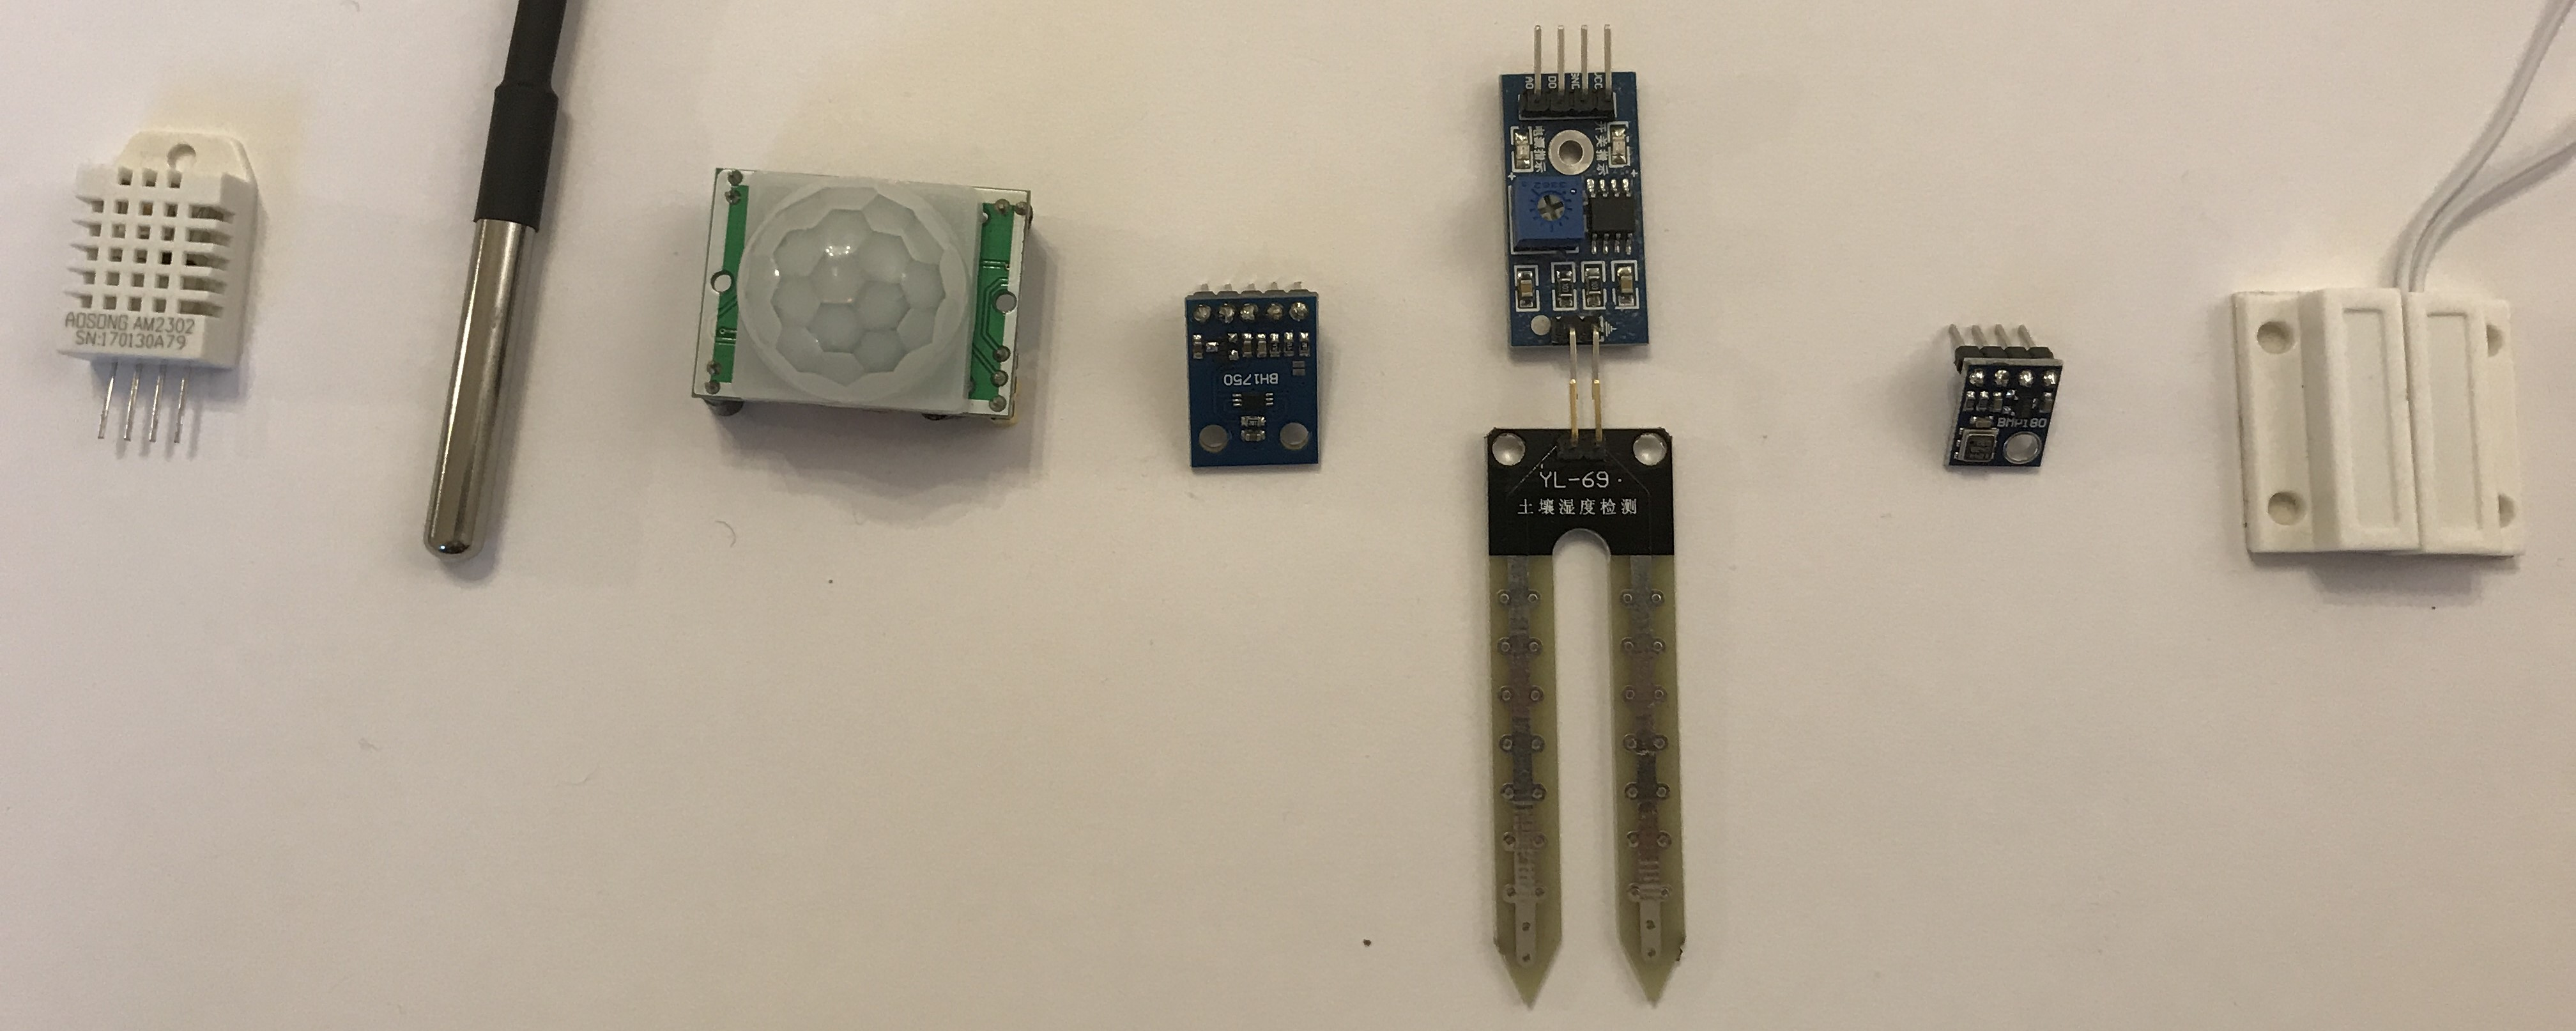
\includegraphics[width=1\textwidth]{bilder/sensoren}
	\caption[Verwendete Sensoren]{Verwendete Sensoren(beginnend von Links): DHT22, DS18B20, PIR-Sensor, BH1750, Bodenfeuchtigkeitssensor, BMP180  und Reed-Kontakt}
	\label{img:verwendeteSensoren}
\end{figure}

\paragraph{DHT11 / DHT22} Bei diesem Sensor handelt es sich um zwei Sensoren, die zur Erfassung von Lufttemperatur und Bestimmung der Luftfeuchtigkeit genutzt werden können. Die beiden Sensoren unterschieden sich nur in der Messgenauigkeit, wobei der DHT22 der genauere der Beiden ist. Die Luftfeuchtigkeit kann bis auf +/- 2\% und die Temperatur auf +/- 0,5 Grad bestimmt werden. Der Wert wird digital zurückgeliefert. Für die Auswertung (siehe Listing \ref{lst:dht22}) der Sensoren wird eine Bibliothek von Adafruit eingesetzt \cite{adafruit2016dht}.

\lstinputlisting[language=C, firstline=348, lastline=350 ,caption={DHT22 Sensorauswertung },label=lst:dht22]{listings/arduinoSensorSenderMesh.ino}

\paragraph{BMP180} Beim BMP180 handelt es sich um einen Luftdrucksensor der über die $I^2C$ Schnittstelle mit dem Arduino verbunden wird. Der Luftdruck kann zwischen 300 und 1100 hPa bestimmt werden \cite{sensortec2013data}. Zusätzlich lässt sich mit diesem Sensor die Temperatur bestimmen, diese Funktion wird allerdings nicht genutzt. Der Sensorknoten bestimmt nur den Luftdruck mit einer Bibliothek von Adafruit (Listing \ref{lst:bmp180}). 
\lstinputlisting[language=C, firstline=364, lastline=368 ,caption={BMP180 Sensorauswertung },label=lst:bmp180]{listings/arduinoSensorSenderMesh.ino}

\paragraph{BH1750} Dieser Sensor wird für die Messung der Beleuchtungsstärke eingesetzt, diese wird in Lux gemessen. Der Sensor unterstützt eine Messung im Bereich zwischen 1 und 65535 Lux, bei einer Auflösung von einem Lux. Der Sensor kann wie der BMP180 über die $I^2C$ Schnittstelle angeschlossen werden. Die Adresse auf der der Sensor erreichbar ist, ist einstellbar. Die Adresse lautet entweder \textit{0x23h} (0 Volt an ADDR- Pin) oder \textit{0x5Ch} (3,3 Volt an ADDR-Pin). 
\paragraph{PIR Sensor} Zur Erkennung von Bewegung wird ein Bewegungsmelder eingesetzt. Der PIR Sensor hat einige Einstellungsmöglichkeiten. Es besteht die Möglichkeit, die Sensitivität und die Dauer des Signals einzustellen. Der PIR Sensor benötigt im Gegensatz zu den vorherigen Sensoren eine Betriebsspannung von 5V. Der Messwert wird einfach mit einem digitalen Eingang gemessen. Eine Nachricht an den Raspberry Pi (Messwertintervall 1min) wird erst nach dem erstmaligen Auslösen des Bewegungsmelders gesendet.
\paragraph{Bodenfeuchtigkeitssensor} Der Bodenfeuchtigkeitssensor verfügt über zwei Ausgänge. Ein Ausgang ist digital und kann mit einem Drehregler direkt am Sensor eingestellt werden. Der Sensor löst beim digitalen Betrieb ab dem definierten Schwellwert aus. Zusätzlich zum digitalen Ausgang liefert der Sensor noch einen analogen Wert, dieser wird dann in einen prozentualen Wert gewandelt (siehe Listing \ref{lst:soilMoisture}). 
\lstinputlisting[language=C, firstline=369, lastline=372 ,caption={Bodenfeuchtigkeit Sensorauswertung },label=lst:soilMoisture]{listings/arduinoSensorSenderMesh.ino}

\paragraph{Reed-Kontakt} Für die Erkennung ob ein Fenster/Tür geschlossen oder geöffnet ist, wurde ein Reed-Kontakt eingesetzt. Dieser fungiert als eine Art Schalter, der ausgelöst wird sobald ein Magnet außerhalb der Reichweite des Reed-Kontaktes ist. Auf dem Sensorknoten sind zwei unterschiedliche Reed-Kontakte installiert. Bei einem kann nur zyklisch überprüft werden ob der Kontakt geschlossen oder geöffnet ist. Der zweite ist an einem Pin mit Interrupt Funktion angeschlossen. Wird dieser ausgelöst wird der Interrupt Service Routine abgearbeitet. Die Nachricht ob ein Reed-Kontakt ausgelöst wurde wird allerdings nur zyklisch abgeschickt. Hierfür wird in jedem Zyklus der Alarm zurückgesetzt und der Interrupt wieder aktiviert, sobald der Reed-Kontakt ausgelöst wurde (siehe Listing \ref{lst:ReedKontakt}). Ein Interrupt wird immer bei wechseln des Signals ausgelöst, das heißt entweder bei einer fallenden oder steigenden Flanke des Signals.
\lstinputlisting[language=C, firstline=383, lastline=389 ,caption={Reed-Kontakt Sensorauswertung },label=lst:ReedKontakt]{listings/arduinoSensorSenderMesh.ino}
\paragraph{DS18B20} Beim DS18B20 handelt es sich um einen Temperatur Sensor, der sowohl die Lufttemperatur messen kann als auch die Bodentemperatur bestimmen kann. Der gesamte Sensor ist in einem wasserdichten Gehäuse. Der Sensor kann über die 1-Wire Schnittstelle angesprochen werden. Dadurch können mehrere Sensoren hintereinander gehängt werden. Diese benötigen eine Datenleitung sowie ein GND und 3,3 V bzw. 5V Leitung. Es können Temperaturen zwischen -55 Grad bis zu 125 Grad mit einer Messgenauigkeit von +/- 0,5 Grad gemessen werden. Jeder Sensor besitzt eine eindeutige und einmalige 64-Bit Seriennummer. An den Sensorknoten können beliebig viele 1-Wire Temperatursensoren angeschlossen werden. Es wird nachdem alle Messwerte von den 1-Wire Sensoren bestimmt wurde jeder Messwert einzeln verschickt (siehe Listing \ref{lst:oneWire}).
\lstinputlisting[language=C, firstline=329, lastline=332 ,caption={1-Wire Sensorauswertung },label=lst:oneWire]{listings/arduinoSensorSenderMesh.ino}

\section{Hardware Design Sensorknoten}
\label{sec:HardwareDesign}
In diesem Unterkapitel werden das Design des Sensorknotens sowie der Produktionsprozess näher betrachtet. Es wird dabei zuerst auf den energiesparenden Sensorknoten, der mit dem Arduino Pro Mini realisiert wurde und anschließend auf den normalen Sensorknoten, der mit dem Arduino Nano eingegangen.
\subsection{Arduino Pro Mini}
\begin{figure}
	\centering
	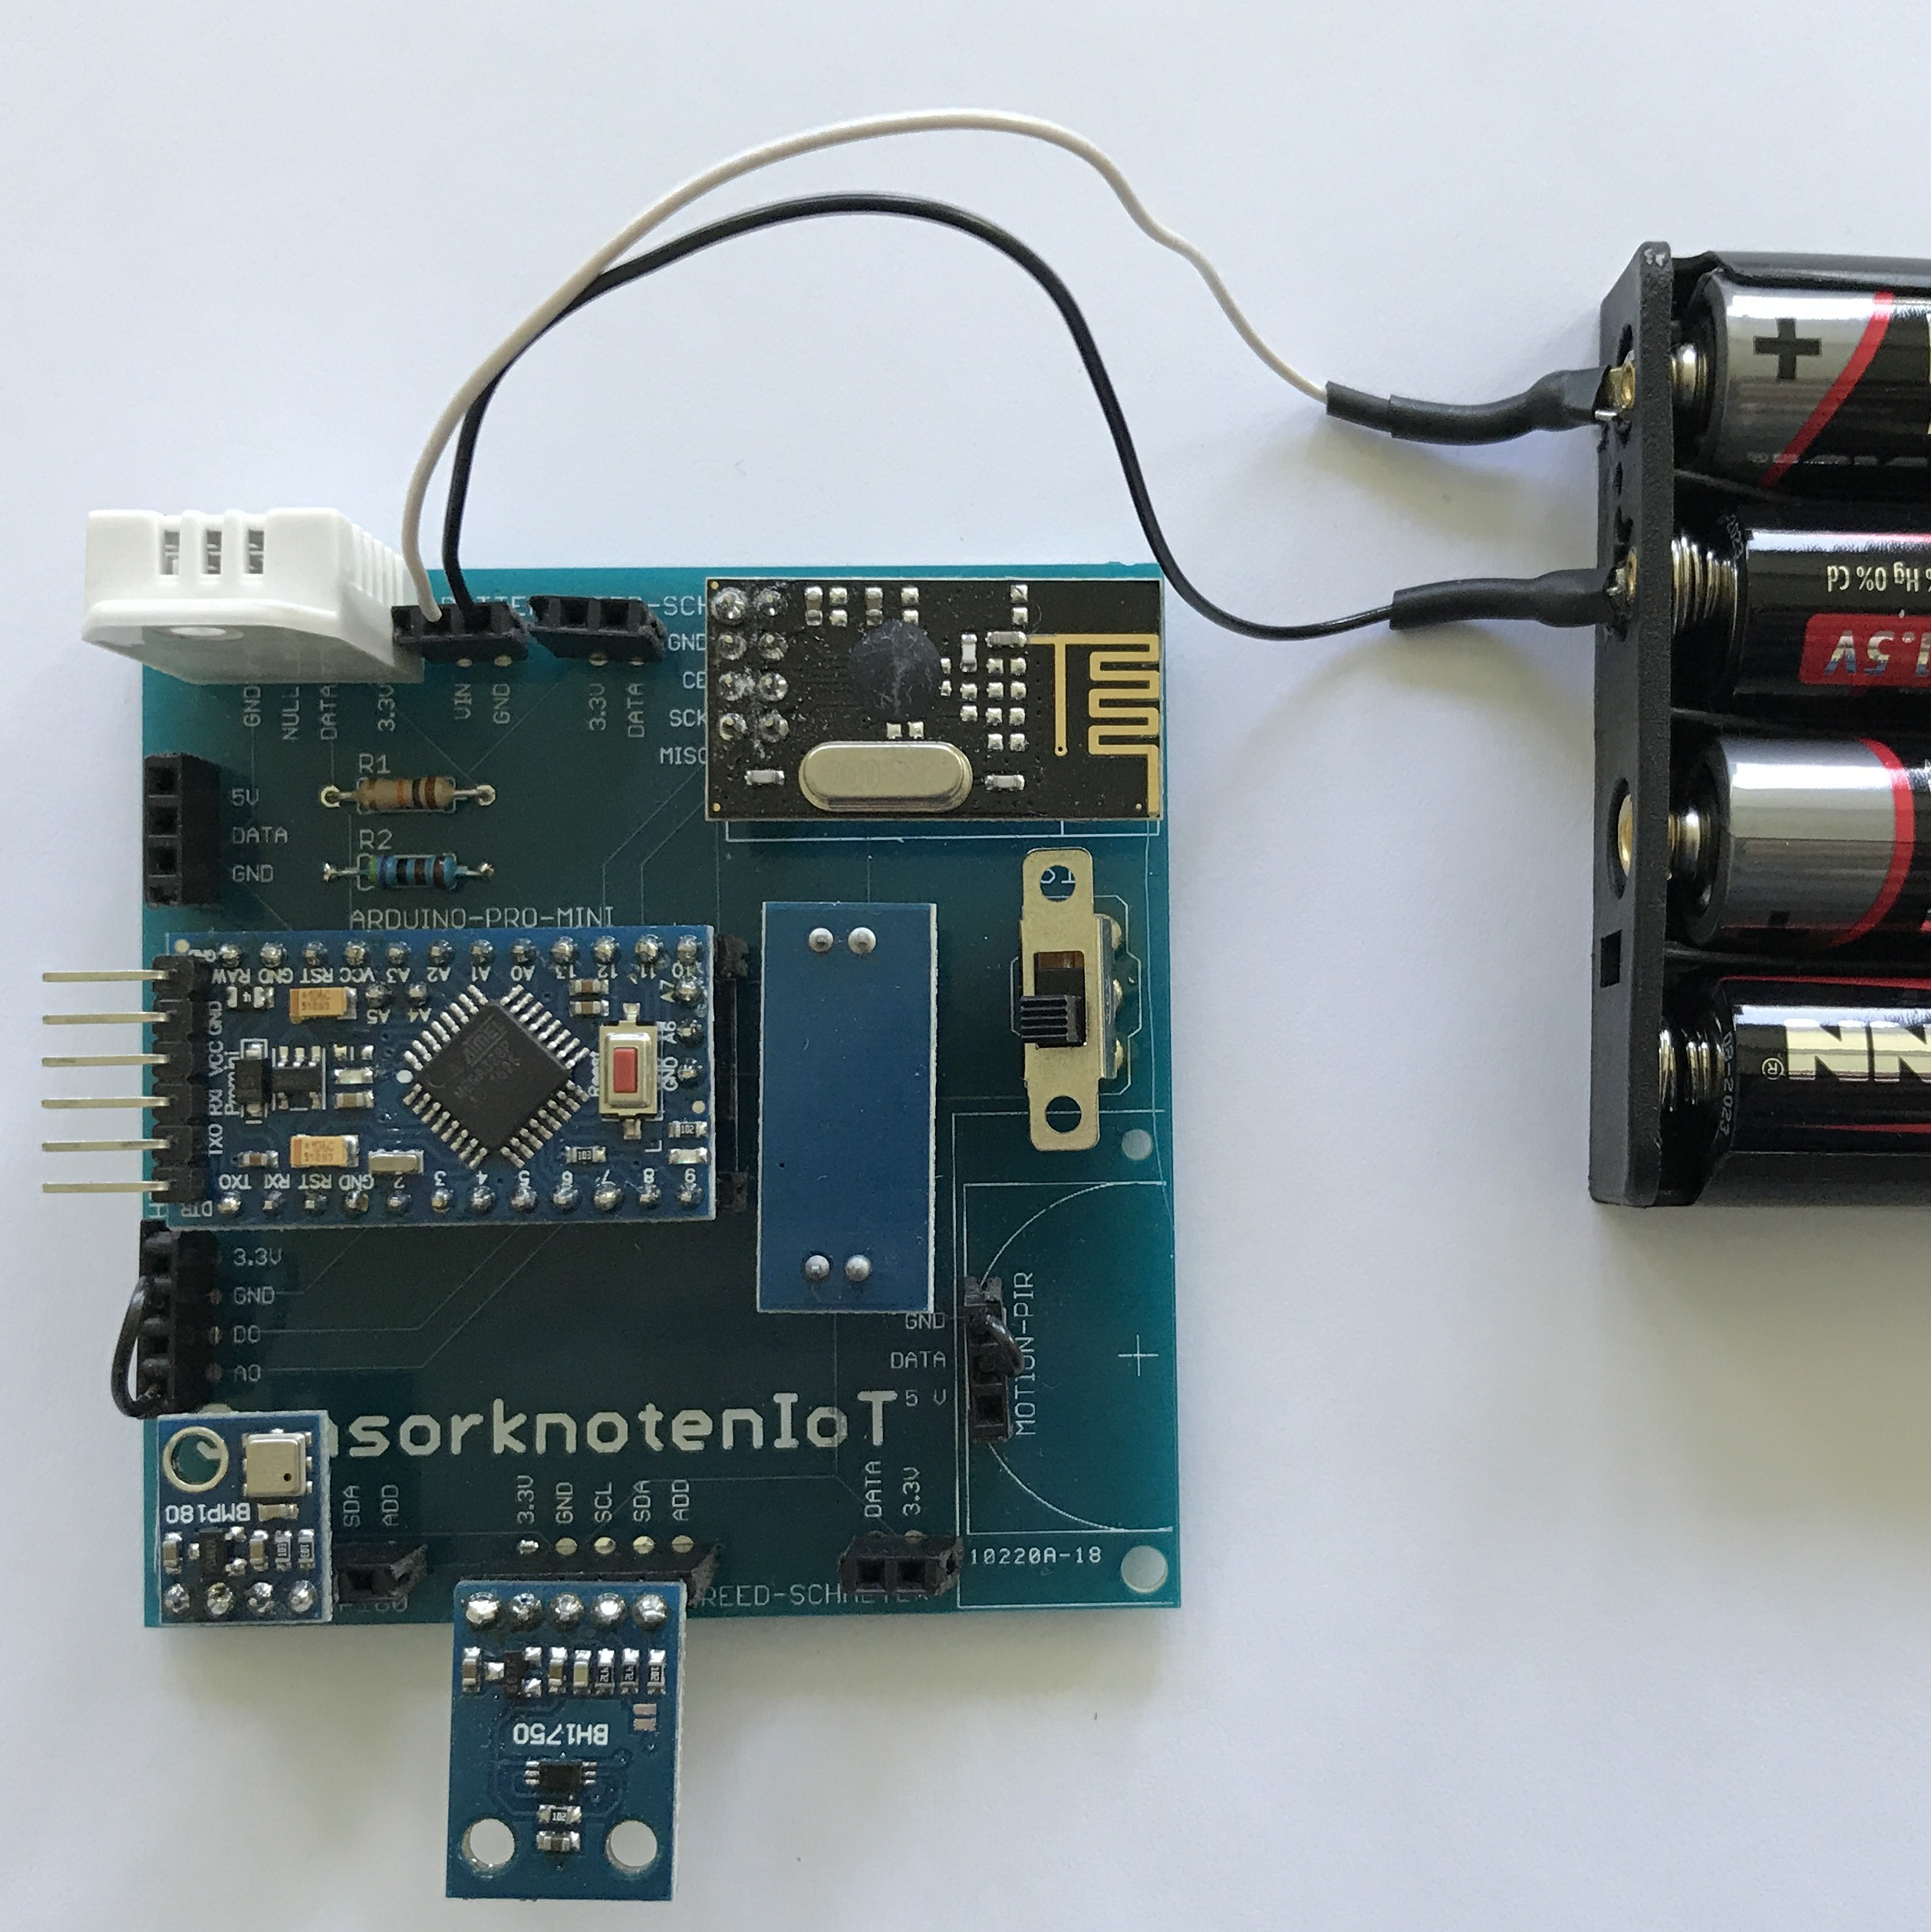
\includegraphics[width=0.6\textwidth]{bilder/mini_cutted}
	\caption[Energiesparender Sensorknoten]{Energiesparender Sensorknoten: bestückt mit verschiedenen Sensoren und einem Arduino Pro Mini}
	\label{img:ArduinoProMini}
\end{figure}
Der energiesparende Sensorknoten wird dauerhaft mit Batterien betrieben. Dieser ist in Bild \ref{img:ArduinoProMini} zu sehen. Der Sensorknoten ist mit einem Arduino Pro Mini bestückt, da dieser energiesparender ist als der Arduino Nano. Sensorknoten lassen sich mit den in Kapitel \ref{sec:VerwendeteSensoren} vorgestellten Sensoren bestücken. Die Sensoren können mit Hilfe von Stiftleisten jederzeit getauscht werden. Nur beim DHT22 bzw. DHT11 haben wir uns entschieden diesen direkt aufzulöten. Der Grundgedanke dabei war, dass jeder Sensorknoten als Mindestanforderung die Temperatur und Luftfeuchtigkeit bestimmen kann. Jeder Sensorknoten besitzt ein nRF24L01 Modul zur Kommunikation mit anderen Sensorknoten oder dem Raspberry Pi.
\paragraph{Spannungsversorgung} Der Arduino Pro Mini verfügt über kein 5V zu 3,3V Wandler, weshalb zusätzlich noch ein Wandler aufgebracht wurde. Dieser 5V zu 3,3V Wandler ist ebenfalls nur mit Hilfe von Stiftleisten aufgebracht. 

Die Spannungsversorgung des Sensorknoten erfolgt mit 4 x 1,5 AA Batterien. Diese liefern gemeinsam eine Spannung von 6V zu Beginn ihrer Betriebszeit. Der Sensorknoten kann bis ca. 4,2V betrieben werden. Die Spannungszufuhr kann mit Hilfe eines Schalters unterbrochen werden. 
\paragraph{Aufgetretene Probleme} Bei der Erstellung des Schaltplans ist ein Fehler bei Sensorschnittstellen für den BMP180 und BH1750 entstanden. Beide Sensoren werden über das $I^2C$ Schnittstelle angesprochen. Hierbei kam es zu einer Vertauschung der 3,3V Leitung und der Masse Leitung. Aus diesem Grund können diese beiden Sensoren nur mit einem Adapter bzw. mit flexiblen Steckbrücken betrieben werden. Die Funktion der Schnittstelle ist davon nicht betroffen. 

Zusätzlich kam es bei der Auswertung der Reed-Kontakte zu zufälligen falschen Werten. Diese konnten behoben werden in dem ein zusätzlicher 10k Ohm Pull Down-Widerstand eingelötet wurde, der das Signal auf Masse zieht.

Um zusätzlich zufällige Werte auszuschließen, wenn kein Bewegungsmelder oder Bodenfeuchtigkeitsmesser angeschlossen ist, wurde eine Steckbrücke genutzt. Diese Steckbrücke verbindet die Datenleitung mit Masse. Durch dieses Verfahren kann einfach überprüft werden ob die Sensoren angeschlossen sind oder nicht.
\label{sec:ArduinoProMini}
\subsection{Arduino Nano}
\label{sec:ArduinoNano}
\begin{figure}
	\centering
	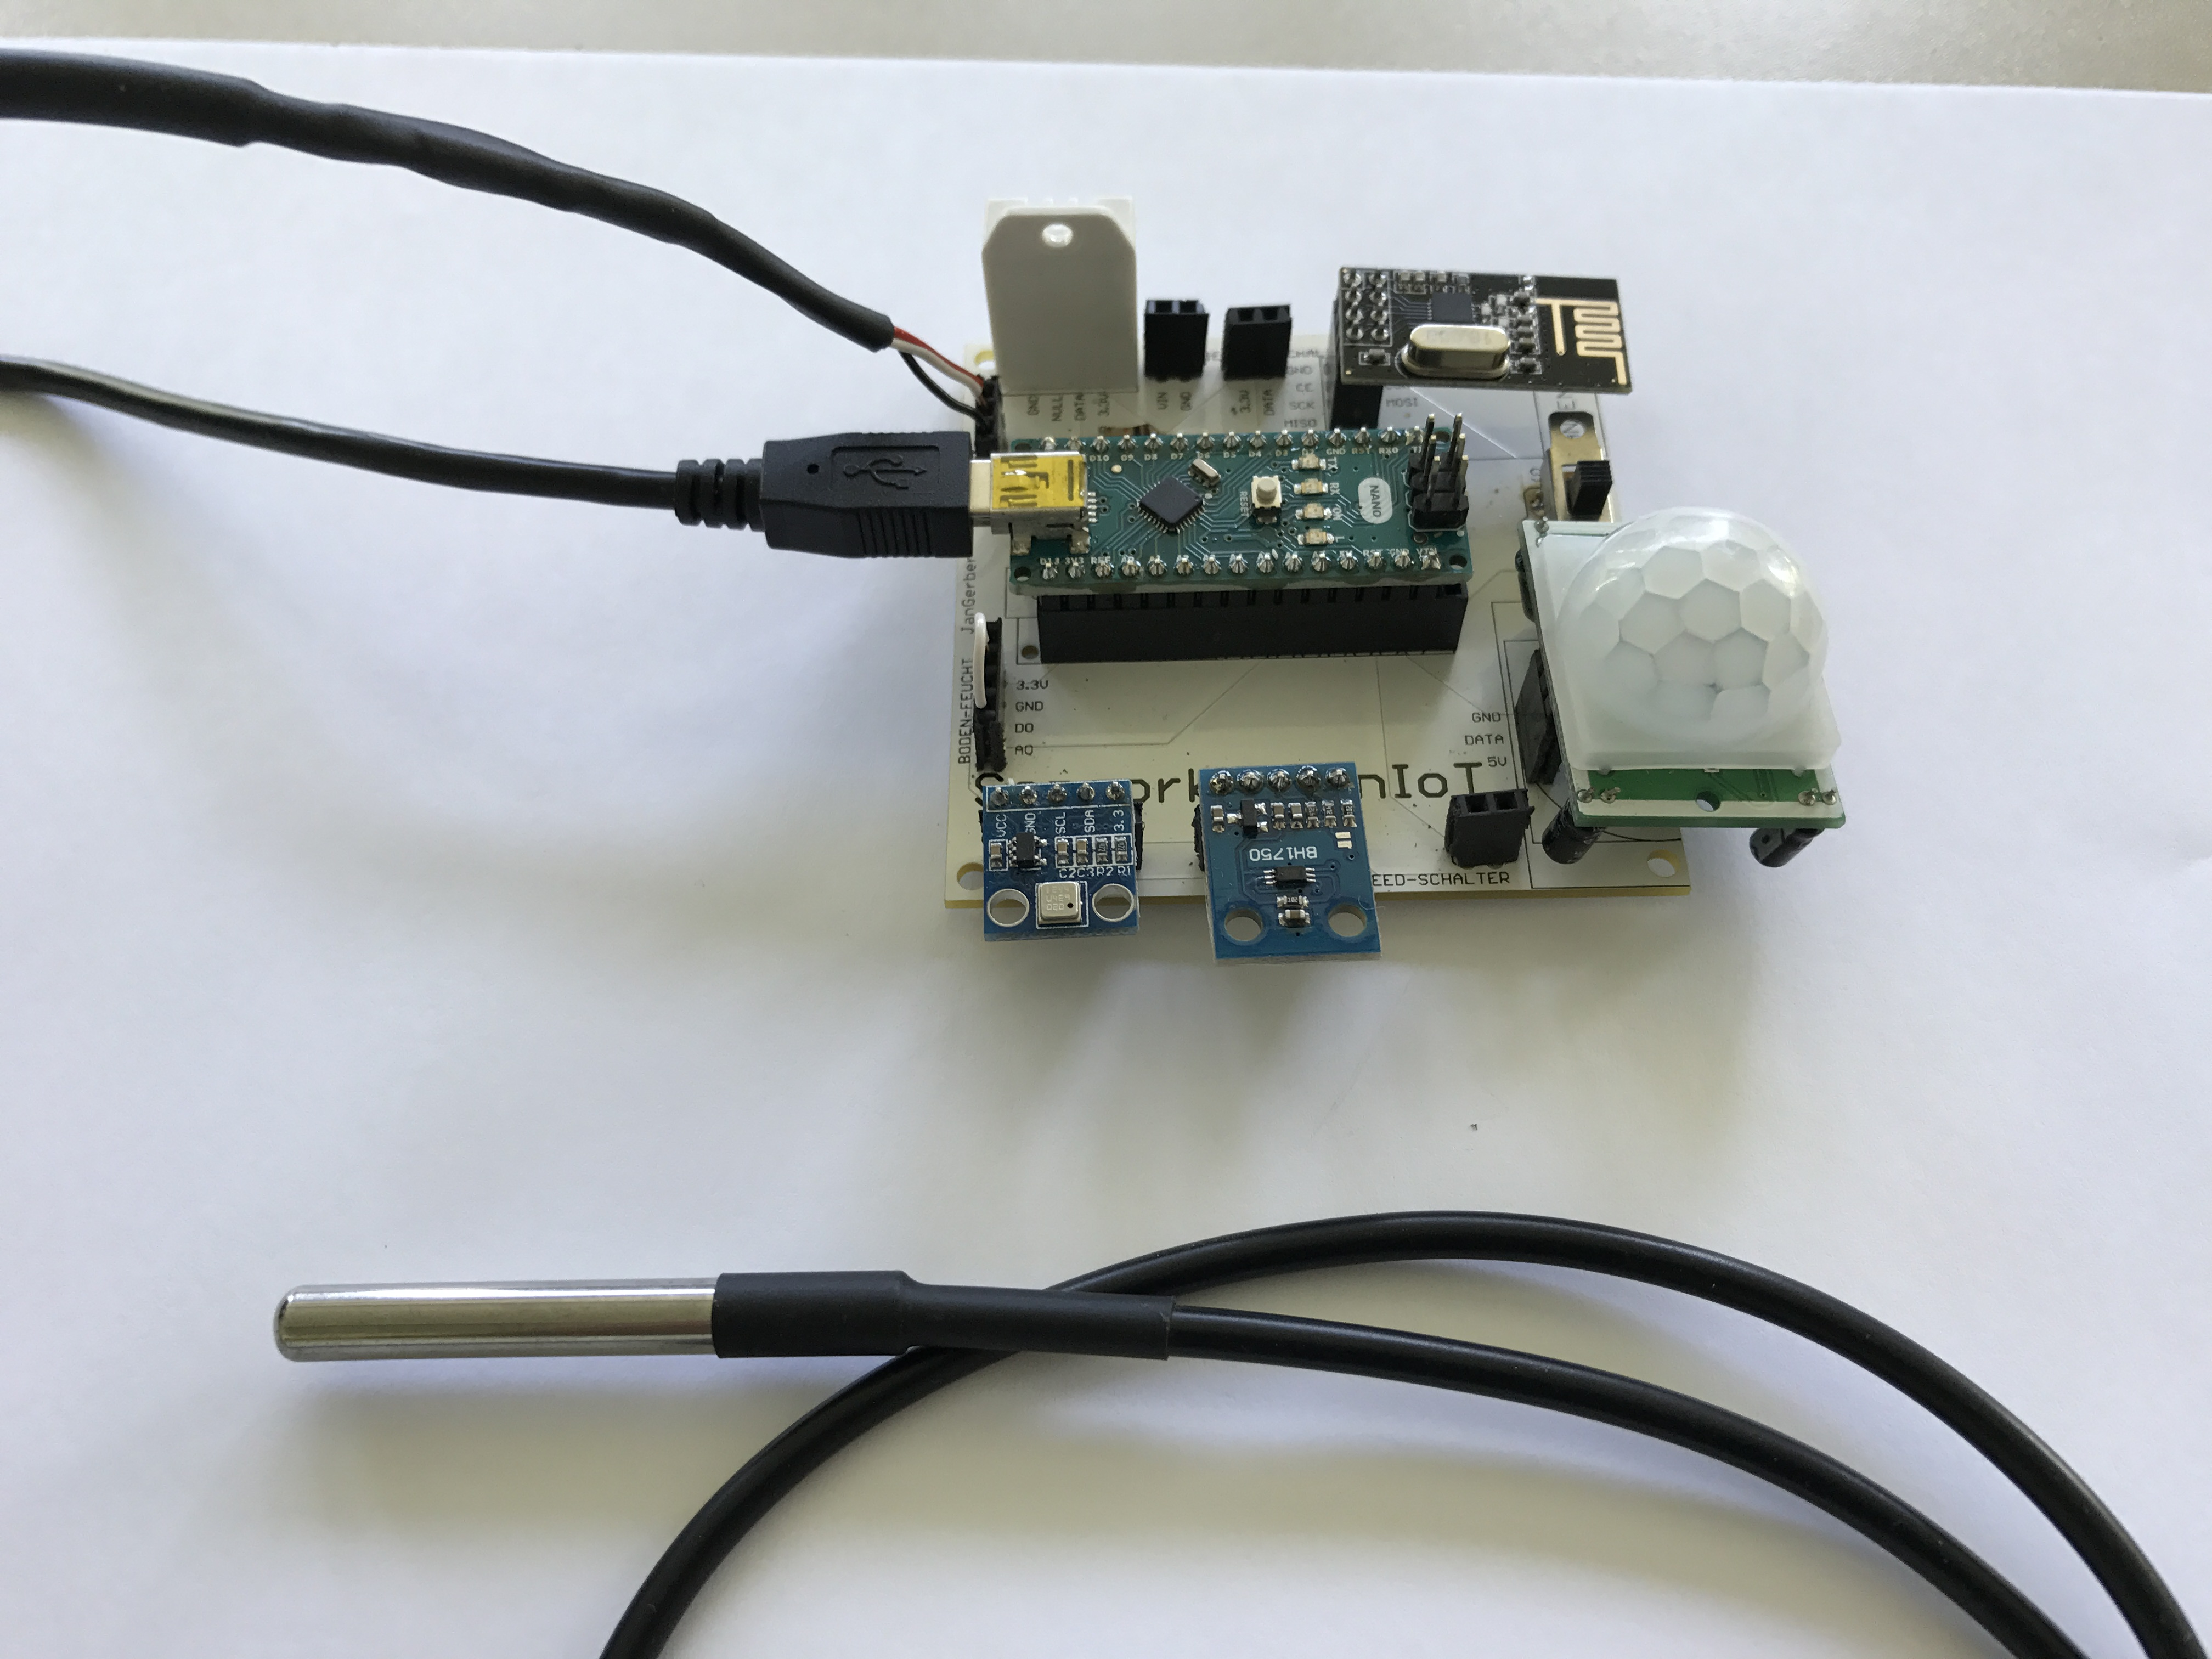
\includegraphics[width=0.6\textwidth]{bilder/SensorknotenArduinoNano}
	\caption[Normaler Sensorknoten]{Normaler Sensorknoten: bestückt mit verschiedenen Sensoren und einem Arduino Nano}
	\label{img:ArduinoNano}
\end{figure}
Der normale Sensorknoten ist mit einem Arduino Nano bestückt. Dieser verfügt über die gleichen Anschlussmöglichkeiten wie der energiesparende Sensorknoten. In Bild \ref{img:ArduinoNano} ist der normale Sensorknoten zu sehen.
\paragraph{Spannungsversorgung} Der normale Sensorknoten kann entweder über die vorhandene USB Schnittstelle betrieben werden oder ebenfalls wie der Arduino Pro Mini über eine externe Stromversorgung, wie zum Beispiel Batterien oder Akkus. Da diese Sensorknoten jedoch deutlich mehr Energie benötigt als der energiesparende Sensorknoten, sollten genügend mAh zur Verfügung gestellt werden. Die externe Stromversorgung kann über einen Schalter ausgeschalten werden. Der Arduino Nano verfügt direkt auf dem Board ein Wandler von 5V zu 3,3V.
\paragraph{Aufgetretene Probleme} Mit dem normalen Board sind die gleichen Probleme hinsichtlich dem Einsatz von Widerständen aufgetreten. Diese Probleme konnten wie beim energiesparende Sensorknoten gelöst werden. Das Sensorknoten Board war allerdings vollständig richtig, was das aufbringen und wechseln von Sensoren deutlich erleichtert.
\subsection{Produktionsprozess der Sensorknoten}
\label{sec:ProduktionsprozessSensornoten}
In diesem Unterkapitel wird auf den gesamten Produktionsprozess eingegangen. Beginnend mit der Entwicklung eines Prototypens, über die Erstellung genauer Schaltpläne und abschließend mit der Bestellung der Platinen, sowie der Bestückung dieser Platinen.
\paragraph{Erstellung eines Prototypen} Um sich in das Thema einzuarbeiten, wurde zunächst ein Prototyp entwickelt (siehe Bild \ref{img:prototyp}. Dieser wurde auf einer einfachen Lochrasterplatine entwickelt. Die einzelnen Komponenten wurden mit Drahtstücken verbunden. Der Löt- und Bestückungsvorgang ging pro Prototyp 2-3 Stunden. Auf dem Prototyp war das Funkmodul, der DHT22 Sensor und eine Sensor mit einer $I^2C$ Schnittstelle aufgebracht. Alle Sensoren konnten in Steckleisten befestigt werden. Dies ermöglichte einen schnellen Austausch, falls ein Sensor ausfallen würde. Für die Erstellung der Prototypen wurde ein handschriftlicher Schaltplan entworfen.
\begin{figure}
	\centering
	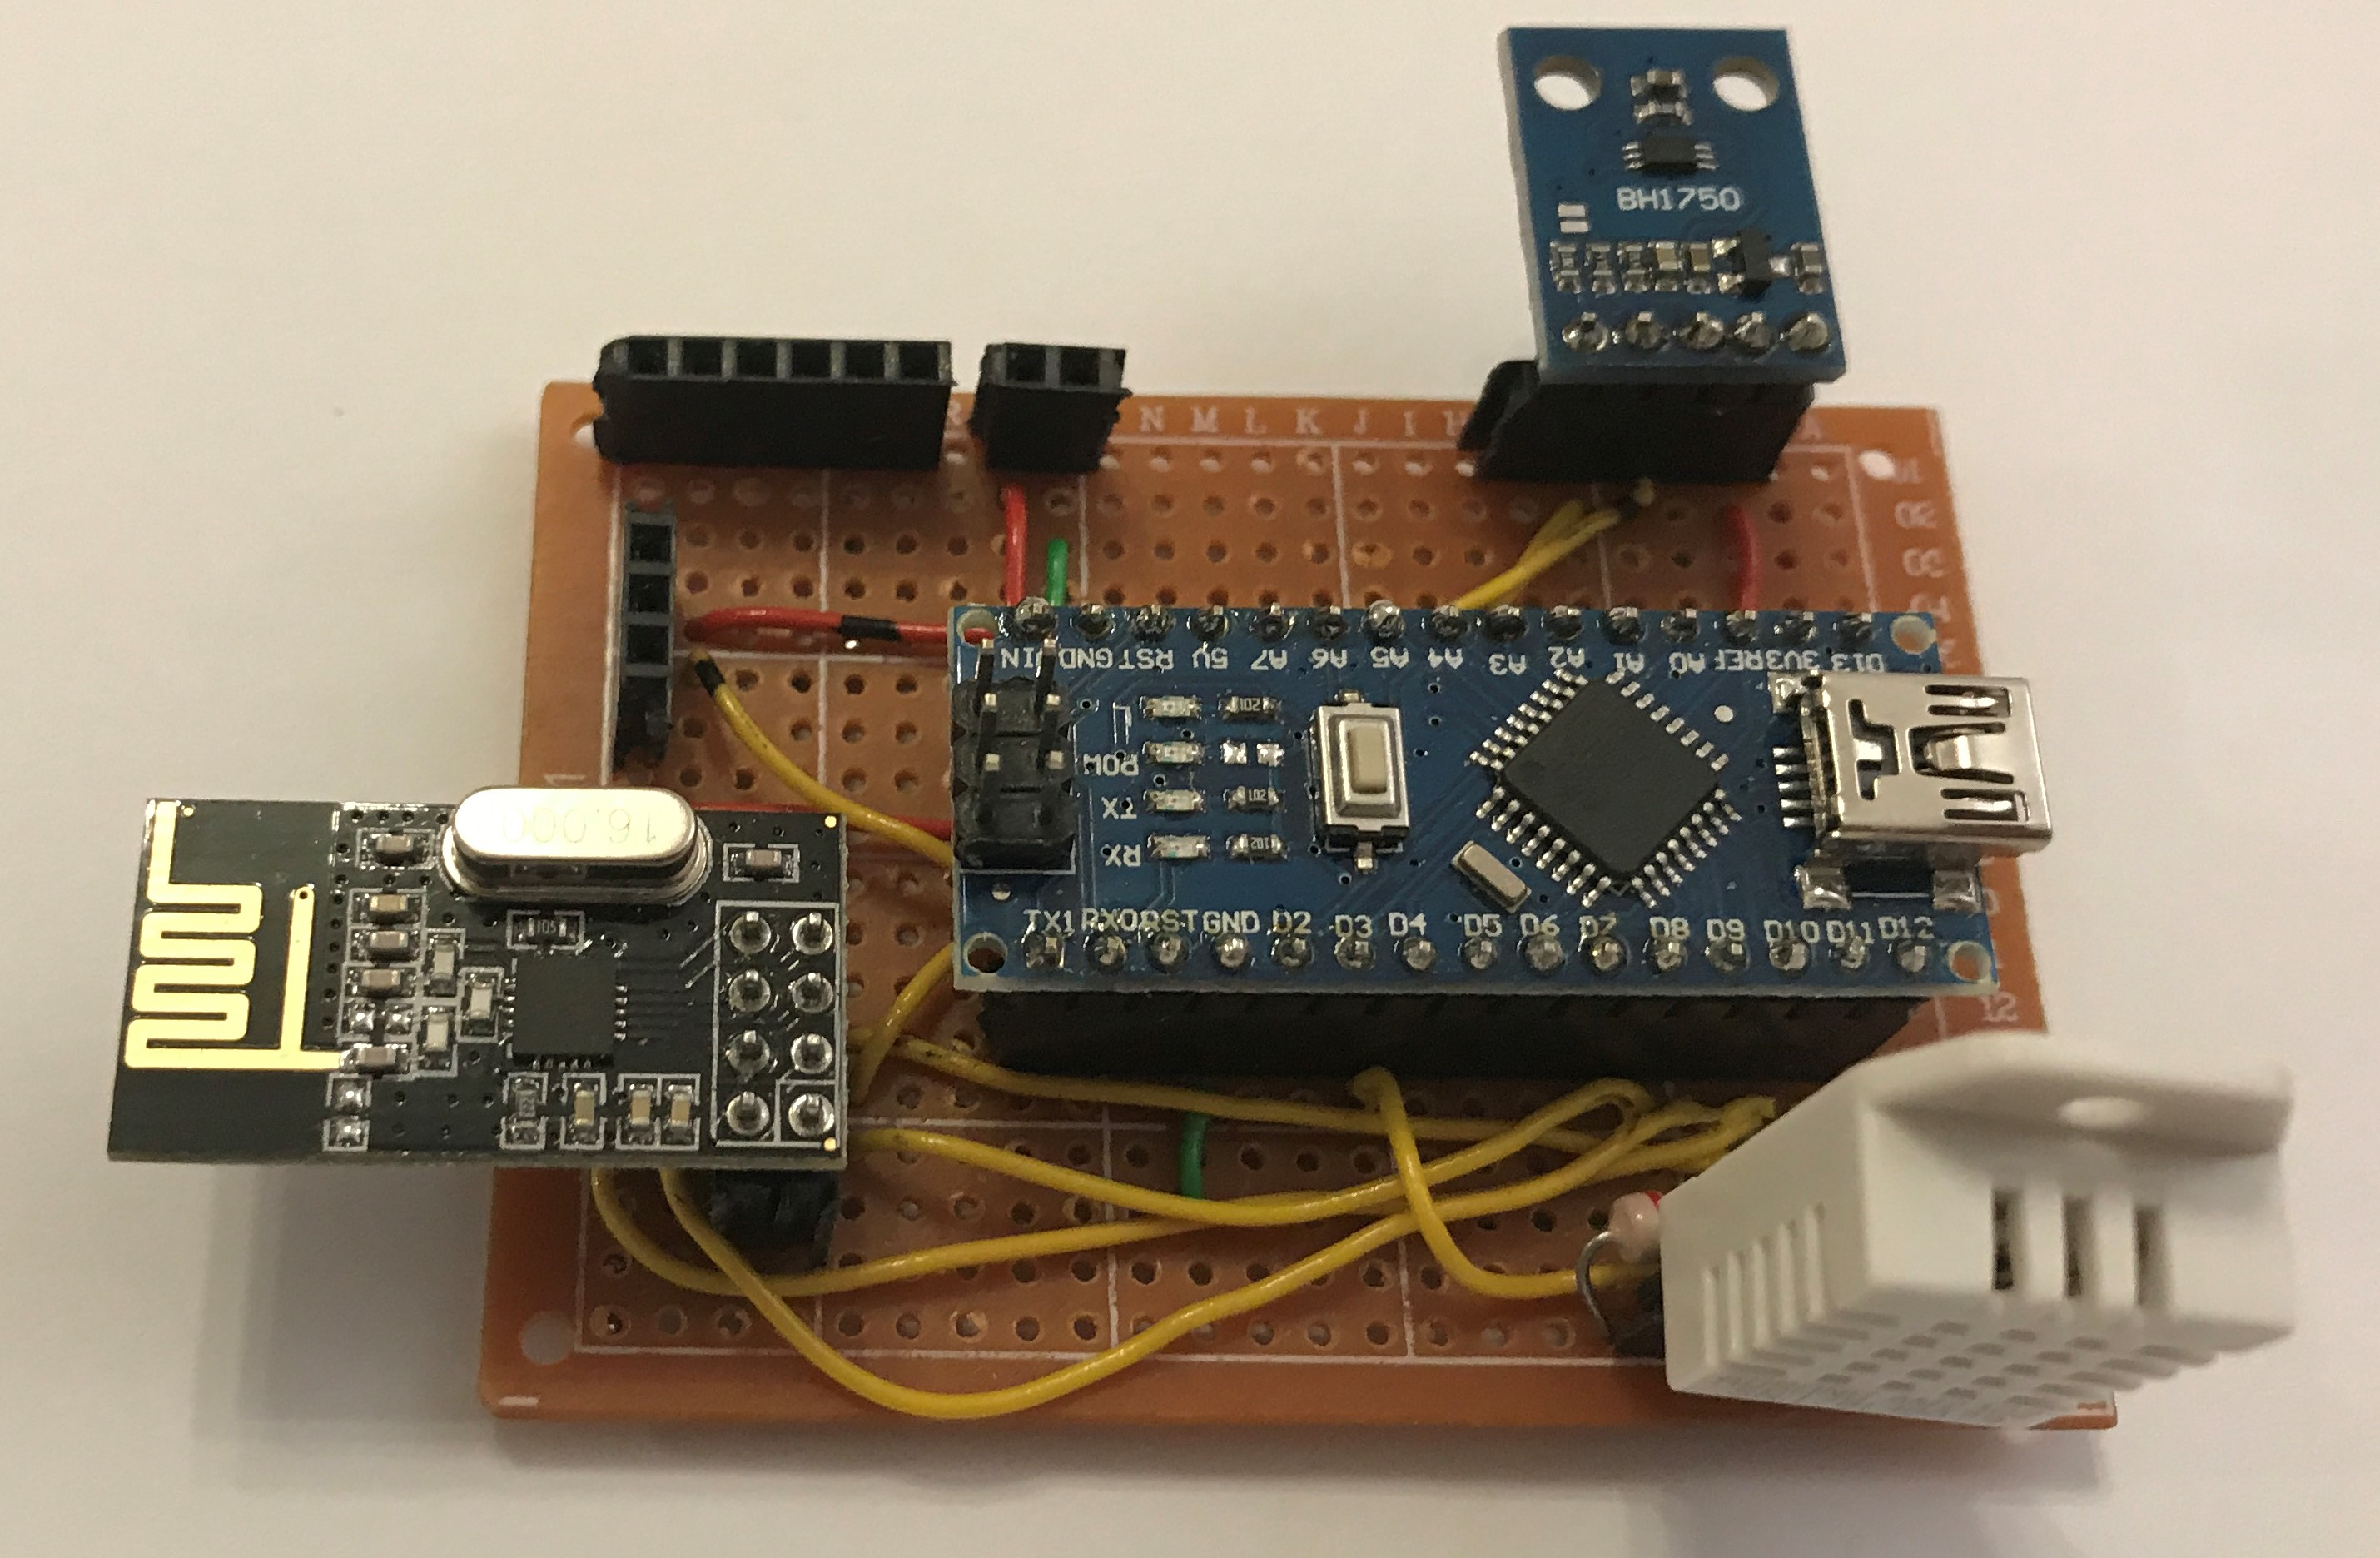
\includegraphics[width=0.6\textwidth]{bilder/prototyp}
	\caption[Prototyp Sensorknoten]{ Prototyp Sensorknoten bestückt mit einem Arduino Nano, DHT22 und dem nRF24l01 Funkmodul und wahlweise mit einem BH1750 oder BMP180}
	\label{img:prototyp}
\end{figure}

\paragraph{Erstellung eines Schaltplans} Nachdem ein funktionsfähiger Prototyp entworfen wurde, konnte ein Schaltplan für den energiesparenden Sensorknoten und den normalen Sensorknoten entwickelt werden. Die Schaltpläne beider Sensorknoten sind im Anhang zu finden. Der Schaltplan wurde komplett entworfen ohne alle Bauteile getestet zu haben. Zusätzlich wurde nur für den normalen Sensorknoten ein Prototypen entworfen, da zum Zeitpunkt der Erstellung des Prototyen die Arduino Pro Mini nicht vorlagen. Der Schaltplan wurde mit Hilfe von Eagle (siehe Kapitel \ref{sec:MesswerterfassungArduino} erstellt.
\paragraph{Erstellung eines Layouts} Eagle bietet die Möglichkeit, nach der Erstellung eines Schaltplans ein Layout für diesen Schaltplan zu entwickeln. Zunächst muss die Größe der Platine festgelegt werden, diese ist bei den Sensorknoten 70 mm * 69 mm. Im nächsten Schritt werden alle Bauteile auf der Platine platziert und positioniert. Die Bauteile wurden so positioniert, dass genügend Platz zwischen den Bauteilen ist.  Anschließend können die Leiterbahnen, mit Hilfe des Autorouters auf der Leiterplatte verlegt werden. Die Leiterbahnen werden nach bereits vorher angegeben Anforderungen (zum Beispiel Abstand und Breite Leiterbahnen) verlegt. Im letzten Schritt wird die Platine noch beschriftet und Bohrlöcher in den Ecken hinzugefügt. So besteht auch die Möglichkeit die Platinen in einem Gehäuse zu befestigen. 
\paragraph{Bestellprozess} Da das Erstellen der Platinen Zeitaufwendig wäre haben wir uns entschieden die Platinen produzieren zu lassen. Nach einem kurzen Vergleich verschiedener Hersteller kamen wir zum Schluss, dass eine Bestellung bei einem chinesischen Hersteller die günstigste Variante ist. Der Hersteller war um den Faktor 10 billiger. Wir haben uns für die Webseite \textit{https://www.seeedstudio.com} entschieden. 
\begin{figure}
	\centering
	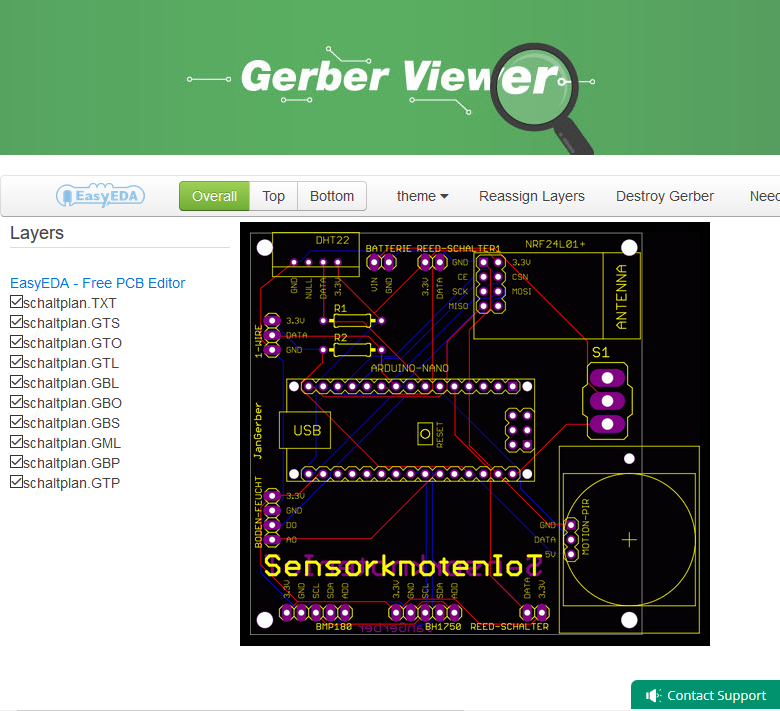
\includegraphics[width=0.6\textwidth]{bilder/gerberViewer}
	\caption{Gerber-Viewer – Seeedstudio.com}
	\label{img:GerberViewer}
\end{figure}

Zunächst musste ein das erstellte Layout in das Gerber-Format exportiert werden. Das Gerber Format enthält alle wichtigen Informationen, die zur Produktion der Platine benötigt werden. Es handelt sich bei diesem Format um eine Art Quasi-Standard. Die Gerber Dateien müssen anschließend gezippt werden und können auf die Webseite hochgeladen werden. Die Webeseite bietet ein Gerber-Viewer um die Leiterplatte nach dem Hochladen noch einmal auf die Korrektheit Zur Überprüfen (siehe Bild \ref{img:GerberViewer}). Dieser Schritt war enorm hilfreich, da so festgestellt werden konnte, dass die Beschriftungen nicht richtig skaliert wurden und Sonderzeichen nicht dargestellt wurden. Eine Abhilfe konnte durch eine Umwandlung der Schriften in eine Vektorgrafik erlangt werden. 

Nachdem die Dateien im Gerber-Format hochgeladen wurden mussten noch einige Angaben zur Platine selbst gemacht werden. Diese Angaben waren für beide Platinen die gleichen mit einer Ausnahme:
\begin{itemize}
	\item Material: FR-4 $\rightarrow$ Verbundwerkstoff aus Epozidharz und Glasfasergewebe
	\item Anzahl Schichten: 2
	\item Größe der Platine: 70 mm x 69 mm
	\item Anzahl an Platinen: 10 Stück
	\item Dicke der Platine: 1,6 mm
	\item Farbe der Platine: Weiß (normaler Sensorknoten), Blau (energiesparender Sensorknoten) 
	\item Oberflächenbehandlung: HASL (Hot Air Solder Leveling mit Zinn/Blei)
	\item Mindestabstand zwischen zwei Leiterbahnen: 0,4 mm
	\item Gewicht der Kupferbahnen: $1 oz/ft^2$  entspricht $300 g/m^2$
	\item Mindestgröße von Bohrlöchern: 0,3 mm
\end{itemize}
Nachdem die Eigenschaften alle festgelegt wurden, wurde der Bestellvorgang fortgesetzt. Im letzten Schritt musste noch die Versandmethode gewählt werden. Wir entschieden uns für die günstigste, die jedoch auch die längste Versanddauer hatte. Der Endbetrag errechnete sich dann aus 10,90 Euro Versandkosten und zweimal 4,51 Euro für die Platinen.

Die Platinen wurden am 14. November 2016 bestellt. Am 22. November 2016 waren die Platinen fertiggestellt und wurden verschickt. Den Versand wurde von Singapore Post und DHL übernommen. Die Ware wurde per Luftfracht verschickt und wurde am 21. Dezember 2016 geliefert. Es gab bei der Zustellung jedoch auch Probleme, da bei dem Bestellvorgang die falsche PLZ angegeben wurde und sich deshalb das Paket um eine Woche verzögerte.
\begin{figure}
	\centering
	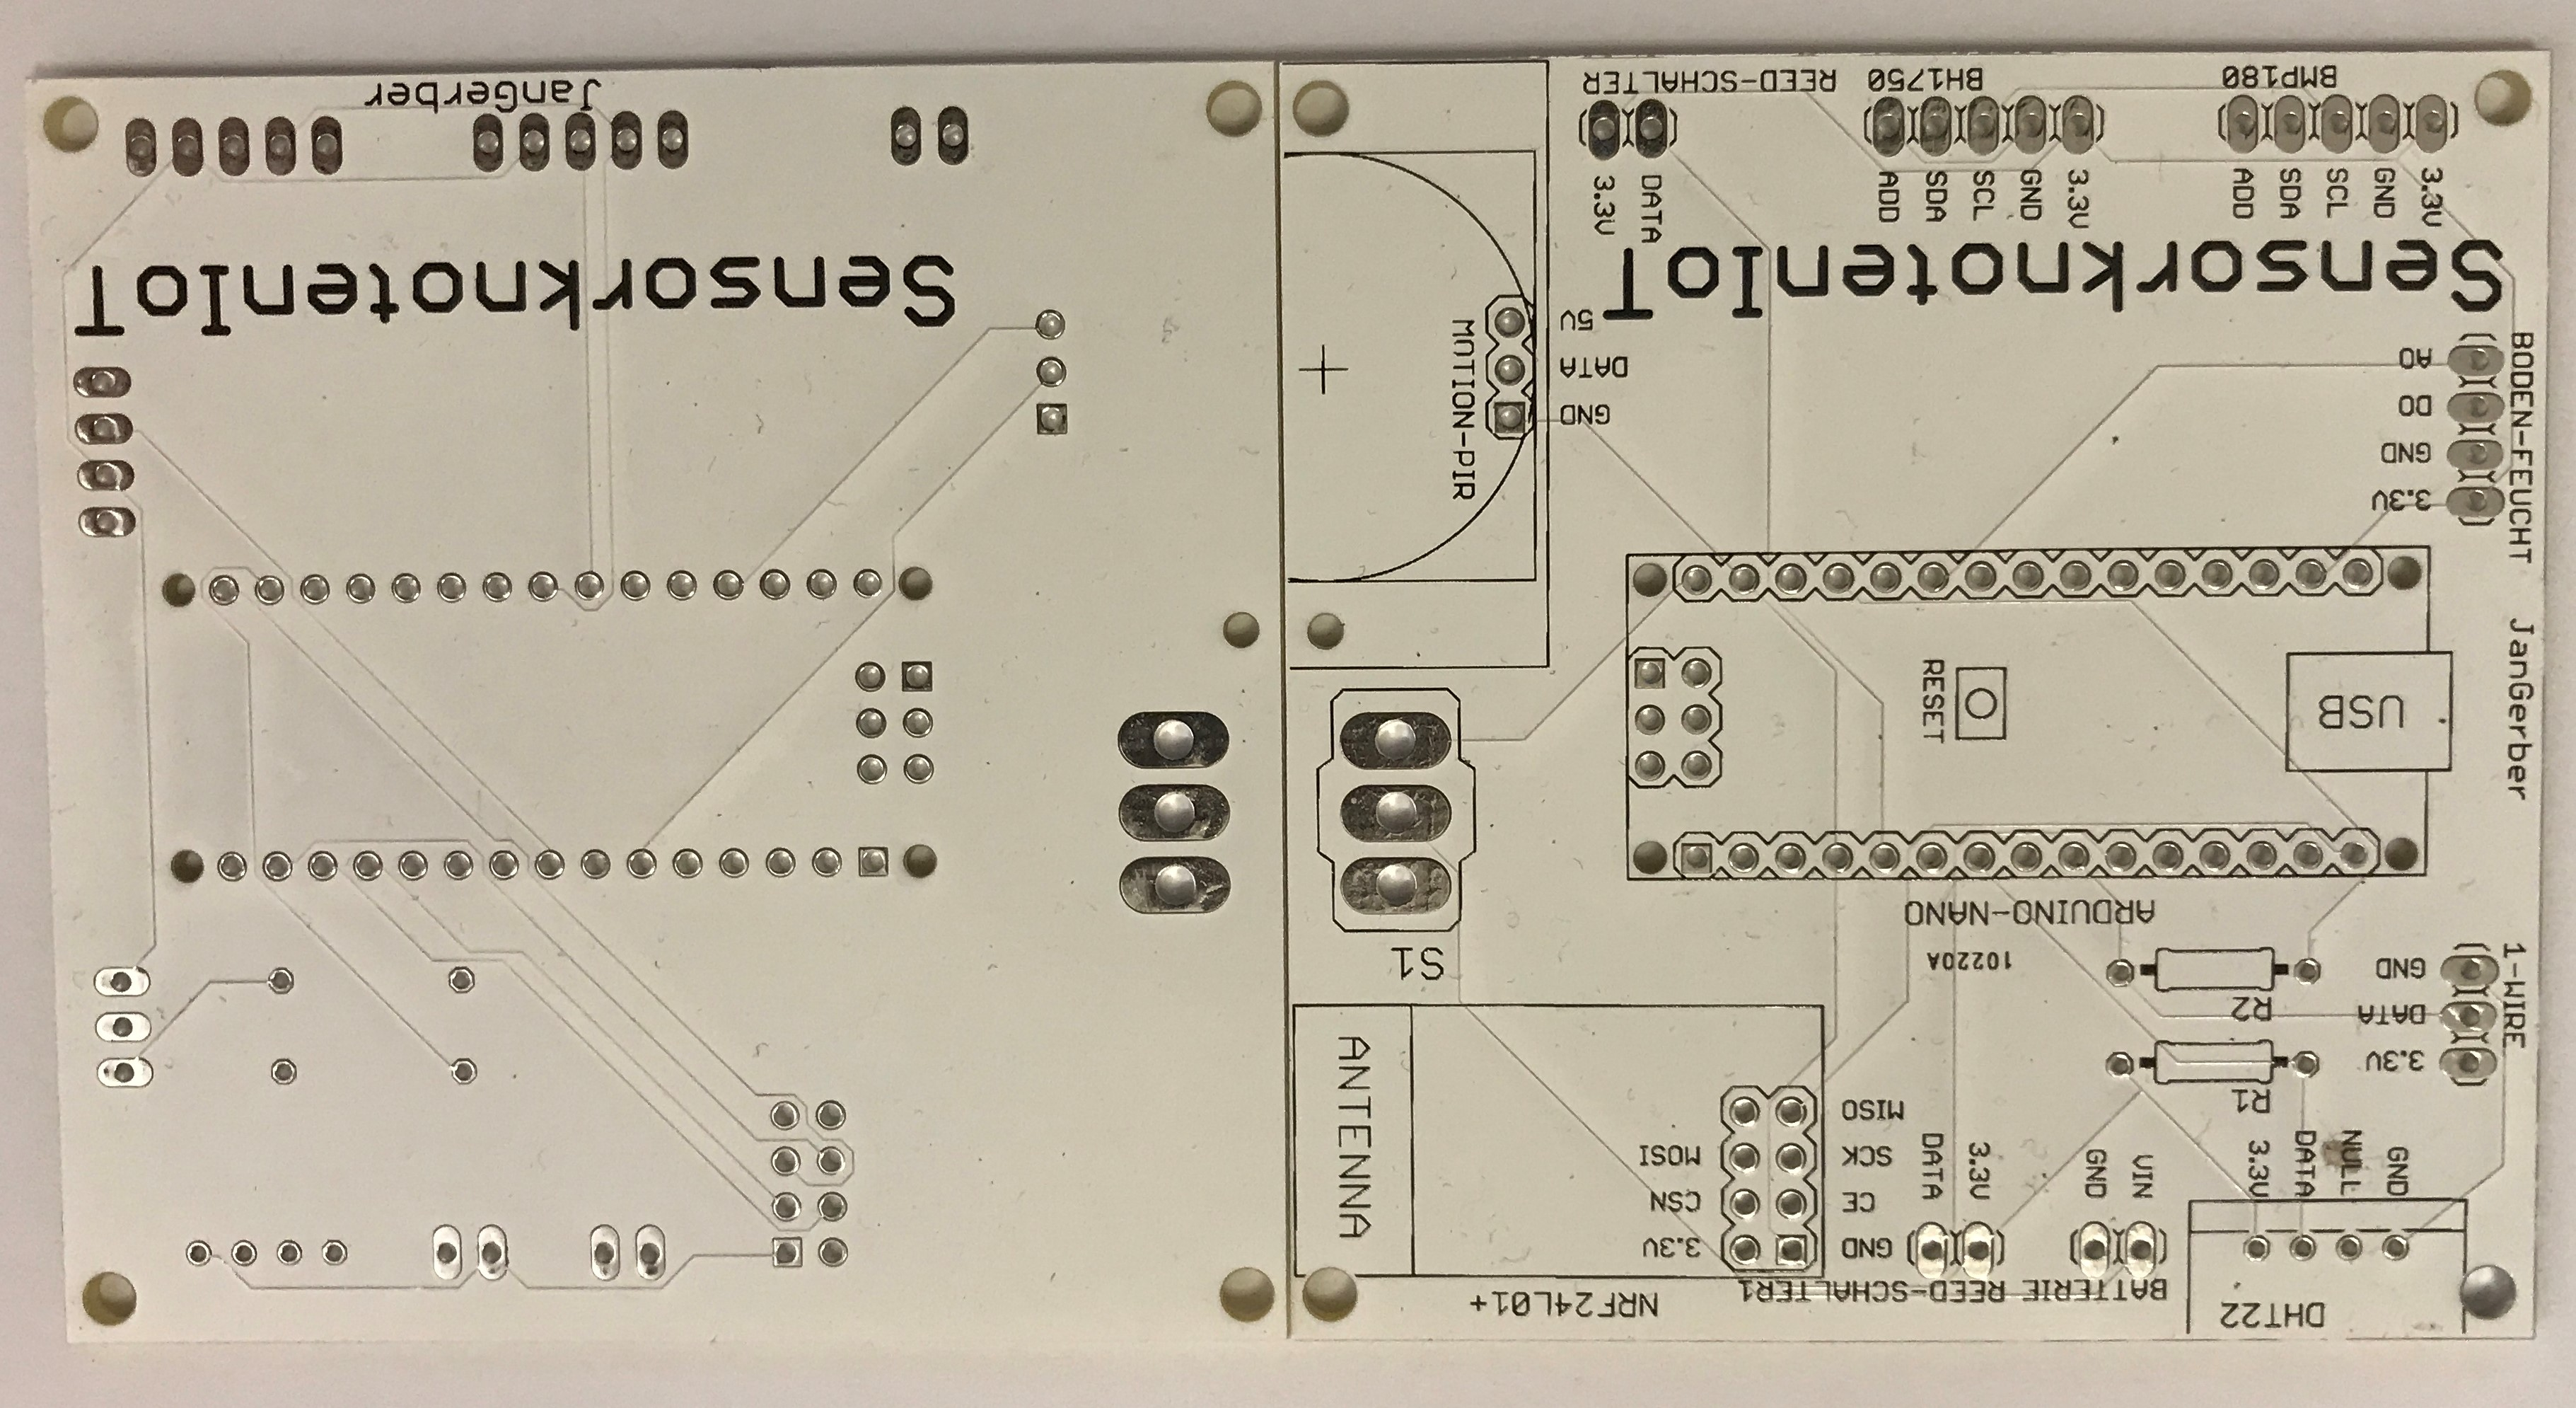
\includegraphics[width=0.6\textwidth]{bilder/platineArduinoNano}
	\caption{Platine für normaler Sensorknoten}
	\label{img:PlatineArduinoNano}
\end{figure}
\begin{figure}
	\centering
	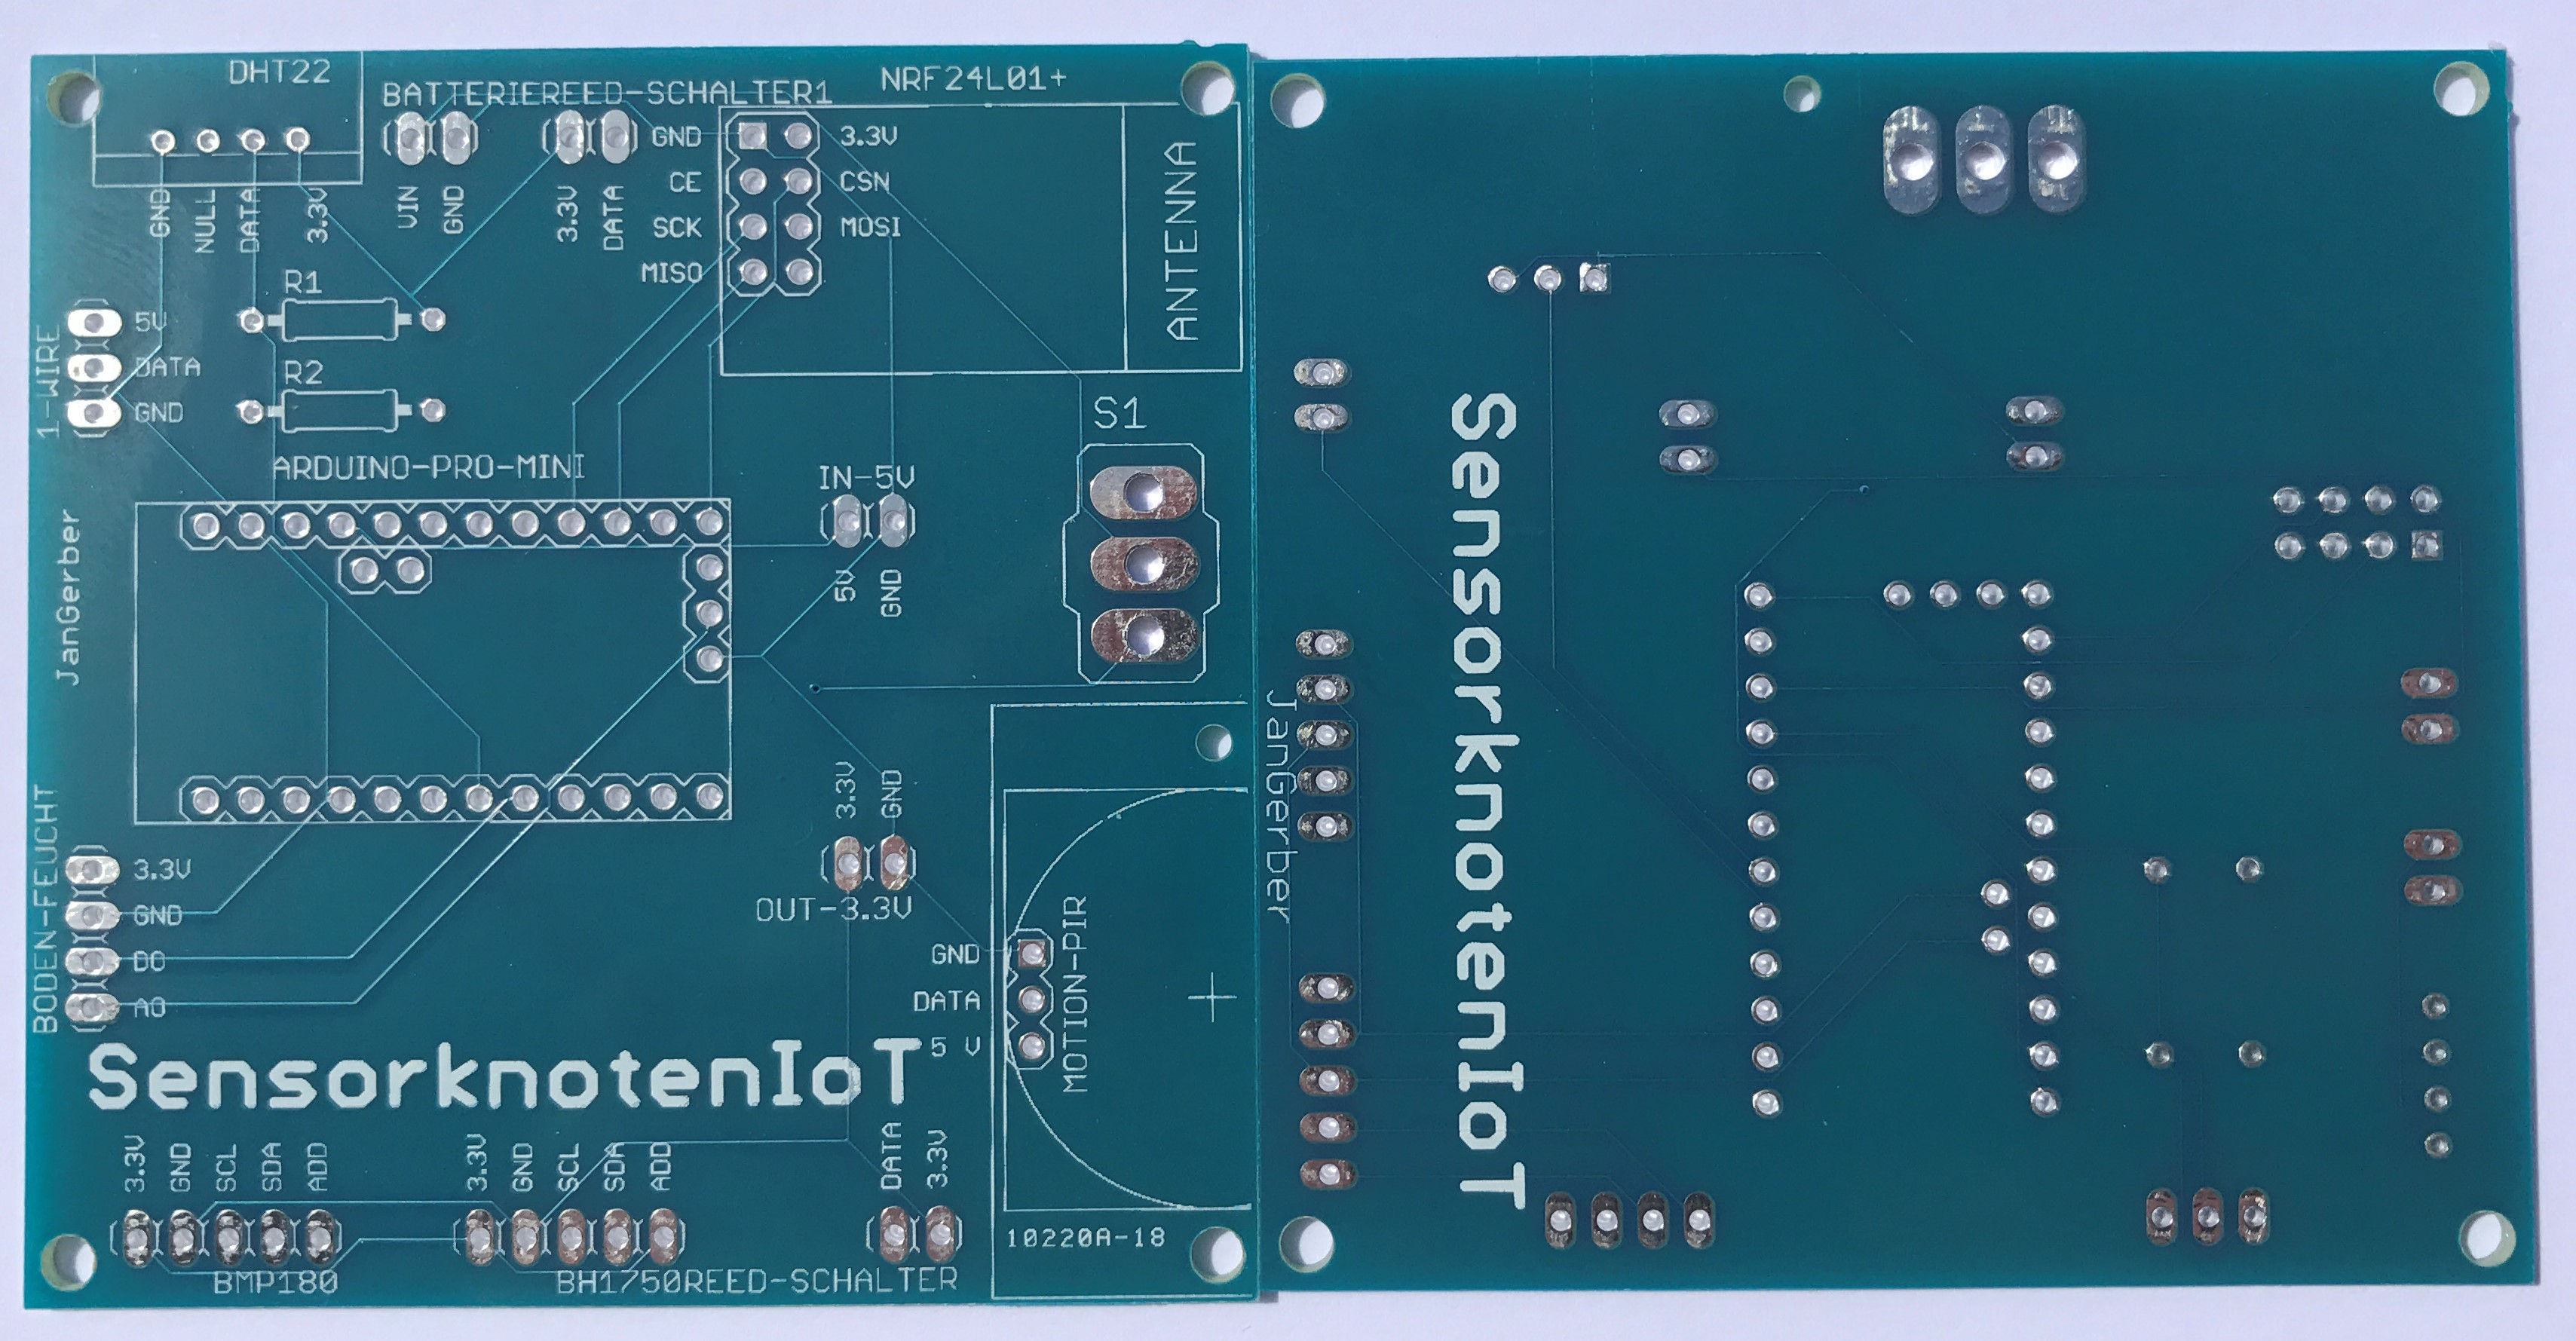
\includegraphics[width=0.6\textwidth]{bilder/platineArduinoProMini}
	\caption{Platine für energiesparender Sensorknoten}
	\label{img:PlatineArduinoProMini}
\end{figure}

\paragraph{Bestückung de Platinen} Die Platinen entsprachen vollständig dem erwarteten Ergebnisses (siehe Bild \ref{img:PlatineArduinoProMini} und \ref{img:PlatineArduinoNano}). Auf die Platinen konnte extrem einfach und schnell die Steckverbindungen, der Schalter, die Widerstände und den DHT22 Sensor aufgebracht werden. Die Produktionszeit einer Platine reduzierte sich so von 3 Stunden auf 10 Minuten. Zusammenfassend kann eine Empfehlung für \textit{Seeedstudio} ausgesprochen werden. Falls das Produkt jedoch kommerziell genutzt werden sollte, darf aufgrund von neuer EU-Richtlinien nur noch bleifreies Lötzinn verwendet werden. 

%\section{Sender}

\section{Raspberry Pi}
Dieses Kapitel beinhaltet die Realisierungen, die den Raspberry Pi betreffen.
\subsection{Verkabelung}
\label{sec:verkabelung_raspi}
Wie eingangs bereits erwähnt, nutzt der Raspberry RF24-Chip. Der Modul existiert in mehreren Ausführungen. Für den Raspberry Pi kommt ein Modul mit externem Antennenanschluss zu Einsatz. Dieses Modul verfügt dank der externen Antenne über eine größere Reichweite. Es hat jedoch auch einen höheren Energiebedarf und die Bauform ist nicht so kompakt wie die Ausführung ohne externe Antenne. Diese zwei Nachteile kommen im vorliegenden Fall beim Raspberry Pi jedoch nicht zum tragen.  

\paragraph{Belegung der GPIO-Pins}
Die Belegung der GPIO-Pins kann man dem Handbuch der RF24-Bibliothek entnehmen:

\begin{table}
    \begin{tabular}{ll|ll}
    \#Pin RF24 & Name auf RF24 & \#Pin Raspberry & Name auf Raspberry \\ \hline
    1                   & GND           & 6                        & GND                \\
    2                   & VCC           & 1                        &  3,3 Volt          \\
    3                   & CE            & 31                       & GPIO22             \\
    4                   & CSN           & 3                        & GPIO8              \\
    5                   & SCK           & 23                       & SCKL(GPIO14)       \\
    6                   & MOSI          & 19                       & MOSI(GPIO12)       \\
    7                   & MISO          & 21                       & MISO(GPIO13)       \\
    8                   & IRQ           & ~                        & ~                  \\
    \end{tabular}
\end{table}

TODO Quelle: \url{https://tmrh20.github.io/RF24/RPi.html}

\subsection{Receiver}
\label{sec:receiver}
\textit{Receiver} meint die Software, die auf dem Raspberry Pi läuft und dort die Nachrichten den Arduinos empfängt. Anfangs war der Receiver in C implementiert. Empfangene Nachrichten (C-Structs) hat das C-Programm geparst (den Bitstrom wieder in einen Struct geschrieben) und in eine Datei geschrieben. Um zu verhindern, dass die Datei unnötig groß wird und um Zugriffe auf die SD-Karte zu verhindern, ging man dazu über eine named Pipe zu nutzen. Da named Pipes nur ein Eintrag im Dateisystem haben, die Speicherstelle jedoch auf den RAM gemappt ist, ist die sehr schnell. Ein zweites Programm in Python hat die empfangenen Daten verarbeitet. 
Da sich die Installation weiterer Bibliotheken für den Raspberry Pi in C als sehr umständlich erwies, entwickelte man einen Receiver in Python. Die Bibliothek stellt hierfür auch Funktionen bereit. 

Zu Beginn erfolgt eine Initialisierung:
\lstset{language=python, numbers=left}
\begin{lstlisting}
radio.begin()
radio.payloadSize = 28
radio.enableDynamicPayloads()
radio.setAutoAck(1)
radio.setDataRate(RF24_250KBPS)
radio.setPALevel(RF24_PA_MAX)
radio.setChannel(90)
radio.setRetries(15, 15)
\end{lstlisting}
Der Aufruf in Zeile 2 legt fest, wie viel Bytes die eintreffenden Nachrichten haben. Zeile 4 sorgt dafür, dass der Raspberry dem Sender den erfolgreichen Empfang sofort automatisch bestätigt. Ferner kann man auch die Datenrate anpassen (Zeile 5) und auch die auch die Empfangs-/Sendeleistung des RF24-Moduls. Im Falle des Raspberry Pis ist die Leitung auf maximal gesetzt. Da er an das Stromnetz angeschlossen ist, ist die Leitungsaufnahme weniger relevant. Das Funkmodul verfügt über 126 Kanäle. Jeder Kanal hat eine Breite von einem Megaherz. Der Kanal ist wählbar über die Funkion \textit{setChannel(CHANNEL)} in Zeile 7. Außerdem kann man definieren, wie oft das Modul versuchen soll, zu senden bevor es eine Bestätigung (Ack) erhält.

Der eigentliche Empfang der Daten erfolgt über den simplen Funktionsaufruf:
\lstset{language=python, numbers=none}
\begin{lstlisting}
receive_payload = readRadio()
\end{lstlisting}



TODO Quelle: \url{https://www.sparkfun.com/datasheets/Components/SMD/nRF24L01Pluss_Preliminary_Product_Specification_v1_0.pdf}   

\subsection{Kodierung}
\label{sec:kodierung}
Das Parsen des empfangenen Bitstroms in einen C-Struct war in Python weiteres nicht mehr möglich. 
Eine der in \ref{sec:anbindung_raspi_arduino} erwähnten Möglichkeiten der Kodierung ist das Erstellen eins Strings und dessen Versand auf dem Arduino. Ein Problem hierbei ist jedoch, das man beachten muss, dass die Länge des Strings variieren kann. Man muss nach der Konkatenation des Strings sicherstellen, dass der String die erwartete Länge hat. Ansonsten kann es zu Problemen bei der Dekodierung beziehungsweise beim Parsen der Daten kommen. Diese Gründe sowie die schlechte Erweiterbarkeit motivierten die Kodierung explizit zu realisieren. 
Eine der in \ref{sec:anbindung_raspi_arduino} erwähnten Möglichkeiten der Kodierung ist das Erstellen eins Strings und dessen Versand auf dem Arduino. Ein Problem hierbei ist jedoch, das man beachten muss, dass die Länge des Strings variieren kann. Man muss nach der Konkatenation des Strings sicherstellen, dass der String die erwartete Länge hat. Ansonsten kann es zu Problemen bei der Dekodierung beziehungsweise beim Parsen der Daten kommen. Diese Gründe sowie die schlechte Erweiterbarkeit motivierten die Kodierung explizit zu realisieren. 

\lstset{language=python, numbers=none}
\begin{lstlisting}
decodedData = base64.b64decode(receive_payload)
\end{lstlisting}
Es kommt Base64 zum Einsatz. Die Kodierung erfordert zwar auf Seite der Arduinos Rechenzeit, die gesendeten Nachrichten sind dadurch jedoch eindeutig zu dekodieren. 

Nach der Dekodierung kann das Programm mit Hilfe des \textit{struct}-Moduls den C-Struct rekonstruieren:  
\lstset{language=python, numbers=none, breaklines=true}
\begin{lstlisting}
destinationAddr, originAddr, lastHopAddr, messageID, stationID, value, unit, timeID = unpack('<hhhhhfhL', decodedData)
\end{lstlisting}
Die deklarierten Variablen erhalten den dementsprechenden Rückgabewert der Funktion \textit{unpack}. Als erstes Argument nimmt sie die Byte order. In diesem Fall ist sie \textit{little-endian}. Anschließend folgen die Datentypen. \textit{h} steht für Short, wobei es sich auf dem Arduino um einen Integer handelt (auf einem x86 würde es sich um einen Short handeln). \textit{f} steht für Float, eine Fließkommazahl und \textit{L} für einen usigned Long, einen long Integer ohne Vorzeichen. 

Quelle TODO \url{https://docs.python.org/2.7/library/struct.html?highlight=struct#module-struct}



\subsection{Hashing}
\label{sec:hashing}
Um später einen eindeutigen Schlüssel für die Datenbank zu haben, nutzt das Programm mehre Attribute. Eine Kombination aus der ID des Arduinos, der Nachrichten-ID und dem hochgezählten Zeitstempel (der Arduino hat keine Echtzeituhr) ist eindeutig, solange keiner dieser Variablen überläuft. Ein Überlauf sollte in ausreichend großer Zukunft liegen. 

\lstset{language=python, numbers=none, breaklines=true}
\begin{lstlisting}
def genearteID_hashed(stationID, messageID, timeID):
    str1 = str(stationID)
    str2 = str(messageID)
    str3 = str(timeID)
    toHash = str1 + str2 + str3
    hashed = hashlib.md5()
    hashed.update(toHash)
return hashed.hexdigest()
\end{lstlisting}
Es kommt ein MD5-Hash zum Einsatz. Dabei handelt es sich um einen 128 Bit langen Hash. 


\subsection{Datenbankanbindung}
\label{sec:db_verbindung}
Das Programm schreibt die empfangenen Daten auch in die Datenbank. Abgesehen von dem Exception-Handling sieht das wie folgt aus: 

\lstset{language=python, numbers=left, breaklines=true}
\begin{lstlisting}
def writeToDatabase(ID_hashed, originAddr, value, unit):
    timeStamp = int(time.time())
    queryCurs.execute('''INSERT IGNORE INTO messwerte (id,originAddr,value,unit,timestamp)
	VALUES (%s,%s,%s,%s,%s)''', (ID_hashed, originAddr, value, unit, timeStamp))
	DBconn.commit()
\end{lstlisting}
Das \textit{IGNORE} in Zeile 3 erspart eine Prüfung, ob die Nachricht bereits verarbeitet ist. Ist die Nachricht in der Datenbank vorhanden, so passiert nichts weiter. Die Datenbank bricht stillschweigend die Transaktion ab. Das entfallen der Prüfung erspart Rechenzeit. Skaliert das gesamte System vertikal (mehr Sensorknoten) , so könnte es andernfalls hier zu Engpässen kommen.   

\subsection{Scheduling}
\label{sec:scheduling}
Das Receiverprogramm startet automatisch wenn der Raspberry Pi bootet. Außerdem sollte der Receiver den Betrieb automatisch wieder aufnehmen nachdem er ungewollter Weise beendet wurde. 
Um das zu realisieren, nutzt man Systemd. Systemd ist ein Initialisierungssytem von Linux. Es ist das erste Programm das beim Boot startet und lädt weitere Programme nach. In diesem Fall auch den Receiver (receiverMesh.py)
\lstset{language=bash, numbers=left, breaklines=true}
\begin{lstlisting}
[Unit]
Description=Receiver
After=multi-user.target

[Service]
Type=simple
ExecStart=/usr/bin/python /home/pi/sensorknoten/receiverMesh.py
Restart=on-abort

[Install]
WantedBy=multi-user.target
\end{lstlisting}
Um einen automatischen Start nach einem Fehler zu gewährleisten bedarf es Zeile 8. Systemd loggt derartige Fälle. So kann man Fehler identifizieren und beheben.

\subsection{Logging}
\label{sec:logging}
Neben Systemd loggt auch das Receiverprogramm. Die Logfile trägt den Namen receiver.log. Das Programm legt sie in dem gleichen Verzeichnis in dem es läuft an. Alle auftretenden Exceptions die nicht zum Programmabsturz führen sollen, finden sich darin wieder.

%\section{Datenverarbeitung}
\section{Webservice}
\label{sec:webservice}
Um von der Clientseite für die Datenrepräsentation die Messdaten zu erhalten, kommt ein Webservice zum Einsatz. Der Webservice ist wie in Kapitel \ref{sec:Topologie} TODO label erwähnt in Python implementiert. Das Microframework \textit{Flask} kam zum Einsatz. Es ermöglicht eine einfache und effektive Implementierung des Webservices. Der Webservice gibt die angefragten Ressourcen im JSON-Format zurück. 

\paragraph{Routen}
Der Webservice verfügt über folgende Routen: 
\begin{enumerate}
\item /mdata/station
\item /mdata/station/$<$int:station$>$
\item /mdata/station/$<$int:station$>$/$<$int:unit$>$
\item /mdata/$<$string:mdatum\_id$>$
\end{enumerate} 
Frägt man auf der ersten Route an, so erhält man eine Liste mit allen in der Datenbank enthaltenen Stationen, zum Beispiel:
\lstset{language=c, numbers=none, breaklines=true}
\begin{lstlisting}
"location": "Wohnzimmer", 
"name": "Station100", 
"originAddr": 100, 
"powerSaving": 0
\end{lstlisting}
Mit Hilfe der zweiten Route kann man alle Messdaten einer Station abrufen. Hier ein Ausschnitt:
\lstset{language=c, numbers=none, breaklines=true}
\begin{lstlisting}
"originAddr": 400, 
"sensor": "Luftdruck", 
"timestamp": 1494414190, 
"unit": 4, 
"unit_name": "hPa", 
"uri": "http://193.196.7.13:8080/mdata/f7bc3361937ee46c33de8aff35196572", 
"value": 993.0
\end{lstlisting}
Über die URI ist die Ressource direkt adressierbar. Dazu kann man die vierte oben genannte Route nutzen, wobei der String \textit{mdatum} der URI entspricht.Die URI ist in der Datenbank die ID. Sie ist auch der Primärschlüssel. Die Erzeugung dieser ID erfolgt wie in \ref{sec:hashing} beschrieben. 
Die dritte Route kann man nutzen um Messdaten einer Größe für einen definierten Zeitraum zu erhalten:
\lstset{language=python, numbers=left, breaklines=true}
\begin{lstlisting}
@app.route('/mdata/station/<int:station>/<int:unit>', methods=['GET'])
@auth.login_required
def get_mdataUnit(station, unit):
    begin = request.args.get('begin')
    end = request.args.get('end')
    anzahlDatenpunkte =  request.args.get('anzahl')

    if begin is not None and end is not None:
        query_result = queryDB_station_interval(station, unit, begin, end)
        query_result =  minimizeData(query_result)
        if len(query_result) != 0:
            return jsonify({'Messdaten':  [make_public_mdatum(data) for data in query_result]})

abort(404)
\end{lstlisting} 
Die Methode nutzt POST-Parameter. In diesem Fall sind die POST-Parameter nicht optional, Zeile 8 prüft, ob sie gegeben sind. Ist die der Fall und die Abfrage aus der Datenbank nicht leer, so springt Zeile 12 aus der Methode raus, ansonsten wirft Zeile 14 den 404 HTTP-Fehler (not found). 

\paragraph{Virtuelle Umgebung}
Um das oben beschriebene Pythonprogramm sicher auf dem Webserver nginx zu veröffentlichen, bedarf es im Idealfall einer virtuellen Pythonumgebung. Diese garantiert unter anderem, dass der User \textit{www-data} (er führt den Webserver aus) nicht unnötig viele Berechtigungen benötigt. Ferner kann die virtuelle Umgebung alle Abhängigkeiten beinhalten. Das Hostsystem muss neben der Installation von Python (ist bei Linux im Regelfall vorinstalliert) keine weiteren Voraussetzungen erfüllen. Im Rahmen dieser Arbeit kommt \textit{virtualenv} zum Einsatz. Mithilfe des Tools \textit{pip} kann man Python-Module (Bibliotheken) in dieser virtuellen Umgebung installieren. Die virtuelle Umgebung enthält auch eine Python-Binary. Ein    

\paragraph{Veröffentlichung auf Webserver}
Um dem Webserver nginx zu ermöglichen, ein Pythonprogramme auszuführen benötigt er einen Applikationsserver. \textit{uWSGI} ist einer dieser Server. Um die Pythonapplikation ausführen zu können ist er unter anderem wie folgt konfiguriert:
\lstset{language=bash, numbers=left, breaklines=true}
\begin{lstlisting}
[uwsgi]
#application's base folder
base = /var/www/restAPI

#python module to import
app = getData_web
module = %(app)

home = %(base)/venv
pythonpath = %(base)
\end{lstlisting}
Zeile 3 definiert das Wurzelverzeichnis des Servers. In Zeile 6 gibt man den Namen der Pythonanwendung bekannt. In Zeile 9 kann man nun die den Pfad nur Python-Binary angeben. Da es sich hier wie oben beschrieben um eine virtuelle Pythonumgebung handelt, ist der Pfad zur Binary \%(base)/venv.
\section{Datenrepräsentation}

\section{Datenbankschema}
\label{sec:db}
Zu Beginn der Entwicklung kam \textit{SQLite} als Datenbankmanagementsystem zum Einsatz. Es stellte sich jedoch heraus, dass es zu Problemen bei gleichzeitigem Zugriff auf die Datenbank kommt. Daher kommt momentan \textit{MySQL} zum Einsatz. MySQL ist weit verbreitetes Datenbankmanagementsystem, ist es Open Source und frei verfügbar. Mit mehreren Datenbankverbindungen kommt es problemlos aus. Das System wird auf dem gleichen Host wie der Webserver für die Datenrepräsentation und der Webservice für die Datenbereitstellung ausgeführt. Dieser externe Server läuft in einer virtuellen Maschine der DHBW Karlsruhe. Das Betriebssystem des Server ist ein Ubuntu-Server. 
\begin{figure}[h!]
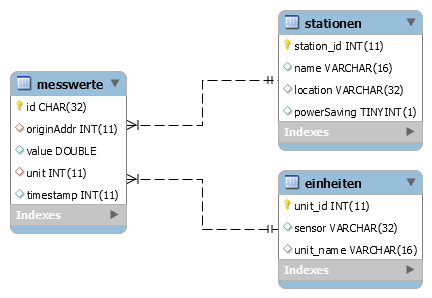
\includegraphics[scale=0.8]{bilder/EERDiagramm} 
\caption{Schema der Datenbank}
\label{Datenbankschema}
\end{figure}   
Die Datenbank beinhaltet drei Tabellen. Bei dem Attribut \textit{id} vom Typ CHAR(32) in der Tablle \textit{messwerte} handelt es sich um die gehashte ID. Diese Tabelle enthält die eigentlichen Messdaten. Die ID dient als Primarykey. Das Attribut \textit{originAddr} gibt an von welchem Sensorknoten (Arduino) das Tupel stammt. \textit{value} gibt den Messwert der entsprechenden Messgröße beziehungsweise Einheit (\textit{unit}) an. Der \textit{timestamp} ist im UNIX-Format. Er zählt die Sekunden seit dem ersten 01.01.1970 hoch. Diese Datumsrepräsentation ist besonders simpel. Da die Arduinos keine Echtzeituhr haben, erstellt der Raspberry Pi beim Empfang den Zeitstempel.
Die Attribute \textit{originAddr} und \textit{unit} sind in \textit{messwerte} sind jeweils Fremdschlüssel. \textit{originAddr} ist Primärschlüssel in der Tabelle \textit{stationen}. Sie dient der Speicherung aller Sensorknoten. Die Tabelle enthält außerdem noch die Spalte \textit{name}, den Standort (\textit{location}) und ein Flag (\textit{powerSavig}), ob es sich um einen energiesparenden Arduino handelt oder nicht.
\textit{einheiten} hat als eindeutigen Primärschlüssel \textit{unit\_id}. In der Tabelle sind alle Messgrößen enthalten. Ein String (VARCHAR(32)) bezeichnet den Sensor (zum Beispiel Luftfeuchte). \textit{unit\_name} repräsentiert die Einheit der Messgröße (zum Beispiel \textit{\%}) 





\chapter{Lösungsbewertung und Fazit}
\section{Vergleich Ist-/Soll-Zustand}
\label{sec:VergleichIstSollZustand}
In diesem Unterkapitel wird der erreichte Ist- Zustand mit dem geforderten Soll-Zustand verglichen. Hierfür werden die gleichen Gliederungspunkte wie in der Problemstellung (siehe Kapitel \ref{sec:SollZustand}) verwendet und hinsichtlich ihrer Realisierung bewertet.
\paragraph{Arduino} Das Ziel war es mit Hilfe des Arduinos verschiedene Sensordaten auszuwerten. Dieser Punkt konnte vollständig erfüllt werden. Die Arduinos können von verschiedenen Sensoren die Messwerte bestimmen. Die Sensoren können je nach Anforderungsprofil an das Sensorknotenboard gesteckt werden. Jeder Sensorknoten hat mindestens den DHT22 oder DHT11 installiert, dieser kann die Temperatur und Luftfeuchtigkeit bestimmen. Alle verwendeten Sensoren wurden bereits in Kapitel \ref{sec:VerwendeteSensoren} vorgestellt.

Ein weiteres Ziel war die Erstellung eines Mesh-Netzes mit Hilfe eines Funkmoduls. Dies wurde mit dem Funkmodul nRF24l01 (siehe Kapitel \ref{sec:MachineZuMachineKommunikation}) realisiert. Die normalen Sensorknoten bauen gemeinsam ein Art Mesh-Netz auf, bei dem über mehrere Knoten hinweg Nachrichten geschickt werden können. Die Nachrichten werden per Broadcast an alle umliegenden Stationen weitergeleitet. Der verwendete Algorithmus wird in Kapitel \ref{sec:MeshAlgorithmus} genauer erklärt.

Als letzter Punkt bei den Arduinos war die Entwicklung eines energiesparenden Sensorknotens. Der entwickelte Sensorknoten verwendet verschiedene Techniken um möglichst wenig Strom zu verbrauchen(siehe Kapitel \ref{ sec:Energiesparmodus}). Der energiesparende Sensorknoten benötigt im Sleep-Modus nur noch 182$\mu$A. Durch diesem geringen Stromverbrauch kann der Sensorknoten über Monate hinweg autark mit Batterien betrieben werden.
\paragraph{Raspberry Pi} Der Raspberry sollte als Gateway zum Internet dienen. Dieser Soll-Zustand wurde vollständig erreicht. Der Raspberry Pi empfängt mit demselben Funkmodul wie die Sensorknoten die Nachrichten der Messwerte. Nach dem Empfangen der Nachricht enkodiert der Raspberry Pi die enthaltene Nachricht und speichert sie in der Datenbank ab. Hierbei werden nur Messwerte von bekannten Sensorknoten und Nachrichten gespeichert die noch nicht in der Datenbank gespeichert wurden. Damit jede Nachricht eindeutig identifizierbar ist wir ein Hash aus der ID des Arduinos, der Nachrichten ID und dem hochgezählten Zeitstemple gebildet (siehe Kapitel \ref{ sec:hashing}. 

Das Programm zum Empfang der Messwerte startet sobald der Raspberrry fertig gebootet ist (siehe Kapitel \ref{sec:scheduling}.
\paragraph{Webservice} Das Soll-Zustand dieses Unterpunktes war es die Sensordaten dauerhaft in einer Datenbank zu speichern und diese Daten mit Hilfe eines REST-Webservice wieder zur Verfügung zu stellen. Dieser Soll-Zustand wurde vollständig erfüllt. Die Implementierung wurde mit Hilfe des Microframework Flask in Python vorgenommen. Der REST-Service stellt vier Routen zur Verfügung die ein Ergebnis in der JSON Notation bereitstellen. Es lassen sich alle Stationen ausgeben, die neusten Messwerte einer Station, die Messdaten einer bestimmten Messgröße über einen bestimmten Zeitraum und die Ressource eines bestimmten Messwertes (siehe Kapitel \ref{ sec:webservice}).
\paragraph{Datenrepäsentation} Als letzte Anforderung war noch die Präsentation der Daten, hierfür sollte ein Frontend entwickelt werden. Das Frontend wurde mit Hilfe verschiedener Webtechnologien entwickelt. Es wurde eine Webseite entwickelt bei dem sich der Nutzer anmelden kann und nach der Authentifizierung eine Übersicht über alle Sensorknoten erhält. Zusätzlich kann sich der Nutzer die aktuellsten Messwerte und zu jedem Sensor ein Kurvendiagramm über ein vom Benutzter definierten Zeitraum ausgeben lassen. Darstellen (siehe Kapitel \ref{sec:Datenvisualiserung}).



\section{Bewertung des Sensorknotens}
-Was kann der Sensorknoten, erreichtes Ziel, Vorteile und Nachteile
\section{Zusammenfassung}
Zeitlich gesehen ging das Entwicklungsteam wie folgt vor:
\begin{itemize}
\item Verbindung zwischen Raspberry Pi und Arduino herstellen (\ref{sec:anbindung_raspi_arduino})
\item Bestückung der Arduinos mit den Sensoren auf der eigen designeten Leiterplatine TDOO REF
\item gleichzeitig die Realisierung der Verarbeitung der Messdaten auf dem Raspberry Pi (\ref{sec:receiver})
\item Erstellen der Messdatenvisualisierung TODO ref und der Messdatenbereitstellung (\ref{sec:webservice}) 
\end{itemize}

Beim Realisieren des Sensorknotens kam es zu einigen Problemen die zu lösen waren. Dazu gehörten unter anderem:
\begin{enumerate}
\item Installation weiterer Bibliotheken auf dem Raspberry Pi
\item Die Kodierung der Nachrichten zwischen Arduino und Raspberry Pi
\item Fehlende Widerstände auf der gefertigten Platine
\item Fehler beim gleichzeitigen Zugriff auf die Datenbank
\item Fehlverhalten der Funkmodule beim Wechseln zwischen Senden und Empfangen
\end{enumerate}

Beim ersten Fehler war es notwendig wie in  \ref{sec:receiver} beschrieben in eine andere Programmiersprache zu wechseln (Python). Die Installation von weiteren Bibliotheken konnte man dort mittels eines Tools einfach vollziehen. 
Um Probleme bei der Kodierung zu eliminieren half es, Nachrichten explizit zu kodieren. Dies geschieht zwar zu Ungunsten der Rechenzeit auf dem Arduino, war jedoch effektiv (\ref{sec:kodierung}). 
Weitere Probleme traten auf in bei der Fertigung der Platinen. Aufgrund eines Planungsfehlers fehlte ein Widerstand TODO ref. Zur Option stand es, die Platinen erneut mit den korrigierten Schaltplänen (siehe Anhang) erneut zu fertigen oder den Fehlenden Widerstand manuell einzulöten. Aufgrund der relativ langen Lieferzeit entschied man sich dafür, die Widerstände einzulöten.
Versuchten mehrere Programme gleichzeitig auf die SQLite-Datenbank zuzugreifen, traten Seiteneffekte auf. Abhilfe schaffte hier der Umstieg auf ein mächtigeres Datenbankmanagementsystem (MySQL, siehe \ref{sec:db}).
In der Bibliothek des RF24-Moduls lauerte ebenfalls ein Fehler. Es war wohl nicht vorgesehen einen Wechseln zwischen Broadcast senden und empfangen zu vollziehen. Die Lösung lag in dem Anpassen der Bibliothek, es ist in TODO ref beschrieben.

\section{Ausblick}
-Registrierung neuer Sensorknoten mittels Webapp
-Routing
-richtiges Mesh
-verschlüsellung
-Datamining
-Aktorknoten

-Auflösung verringern von Daten

Bei der Realisierung dieses Projekts kamen Ideen für die Fortsetzung der Arbeit auf. So wäre eine benutzerfreundliche Möglichkeit weitere Sensorknoten zu registrieren mit Sicherheit ein gefragtes Feature. Man könnte dies mit eines Webapplikation umsetzten.
Der Vorhanden "Mesh-Algorithmus" ist in Zukünftigen Arbeiten ersetzbar durch einen Mesh-Algorithmus wie er in der Literatur definiert ist. Dazu kann man beispielsweise einen entsprechenden RFC implementieren. In diesem Zuge ist es auch möglich eine Routing-Metrik für das neu implementierte Protokoll zu designen und die Datenpakete zu verschlüsseln. 

Die gesammelten Sensordaten sind auch als Basis für Dataminig nutzbar

Ferner kann auch der Gegenspieler zum Sensorknoten realisiert werden, ein Aktorknoten.

 

 

% #################################################



%\include{changelog}

\singlespacing %Literaturverzeichnis wieder 1-facher Zeilenabstand.

\addcontentsline{toc}{chapter}{Literaturverzeichnis}

% Haben Sie das "biblatex"-Paket nicht installiert, benutzen Sie folgendes:
% Ohne das "biblatex"-Paket (s. bericht.sty) produziert folgendes
% "deutsche" Zitate in Literaturverzeichnissen gemaß der Norm DIN 1505,
% Teil 2 vom Jan. 1984.
% Die Zitatmarken werden alphabetisch nach Verfassern
% sortiert und sind durch abgekürzte Verfasserbuchstaben plus
% Erscheinungsjahr in eckigen Klammern gekennzeichnet.

% \bibliographystyle{alphadin}
% \bibliography{bericht}

%%%%%%%%%%%%%%%%%%%%%%%%%%%%%%%%%%%%%%%5
% BIBLATEX
% Benutzt man das "biblatex"-Paket, muß man folgendes schreiben:
\def\refname{Literaturverzeichnis}
\printbibliography    

%%%%%%%%%%%%%%%%%%%%%%%%%%%%%%%%%%%%%%%5

% Ab hier beginnt der Anhang


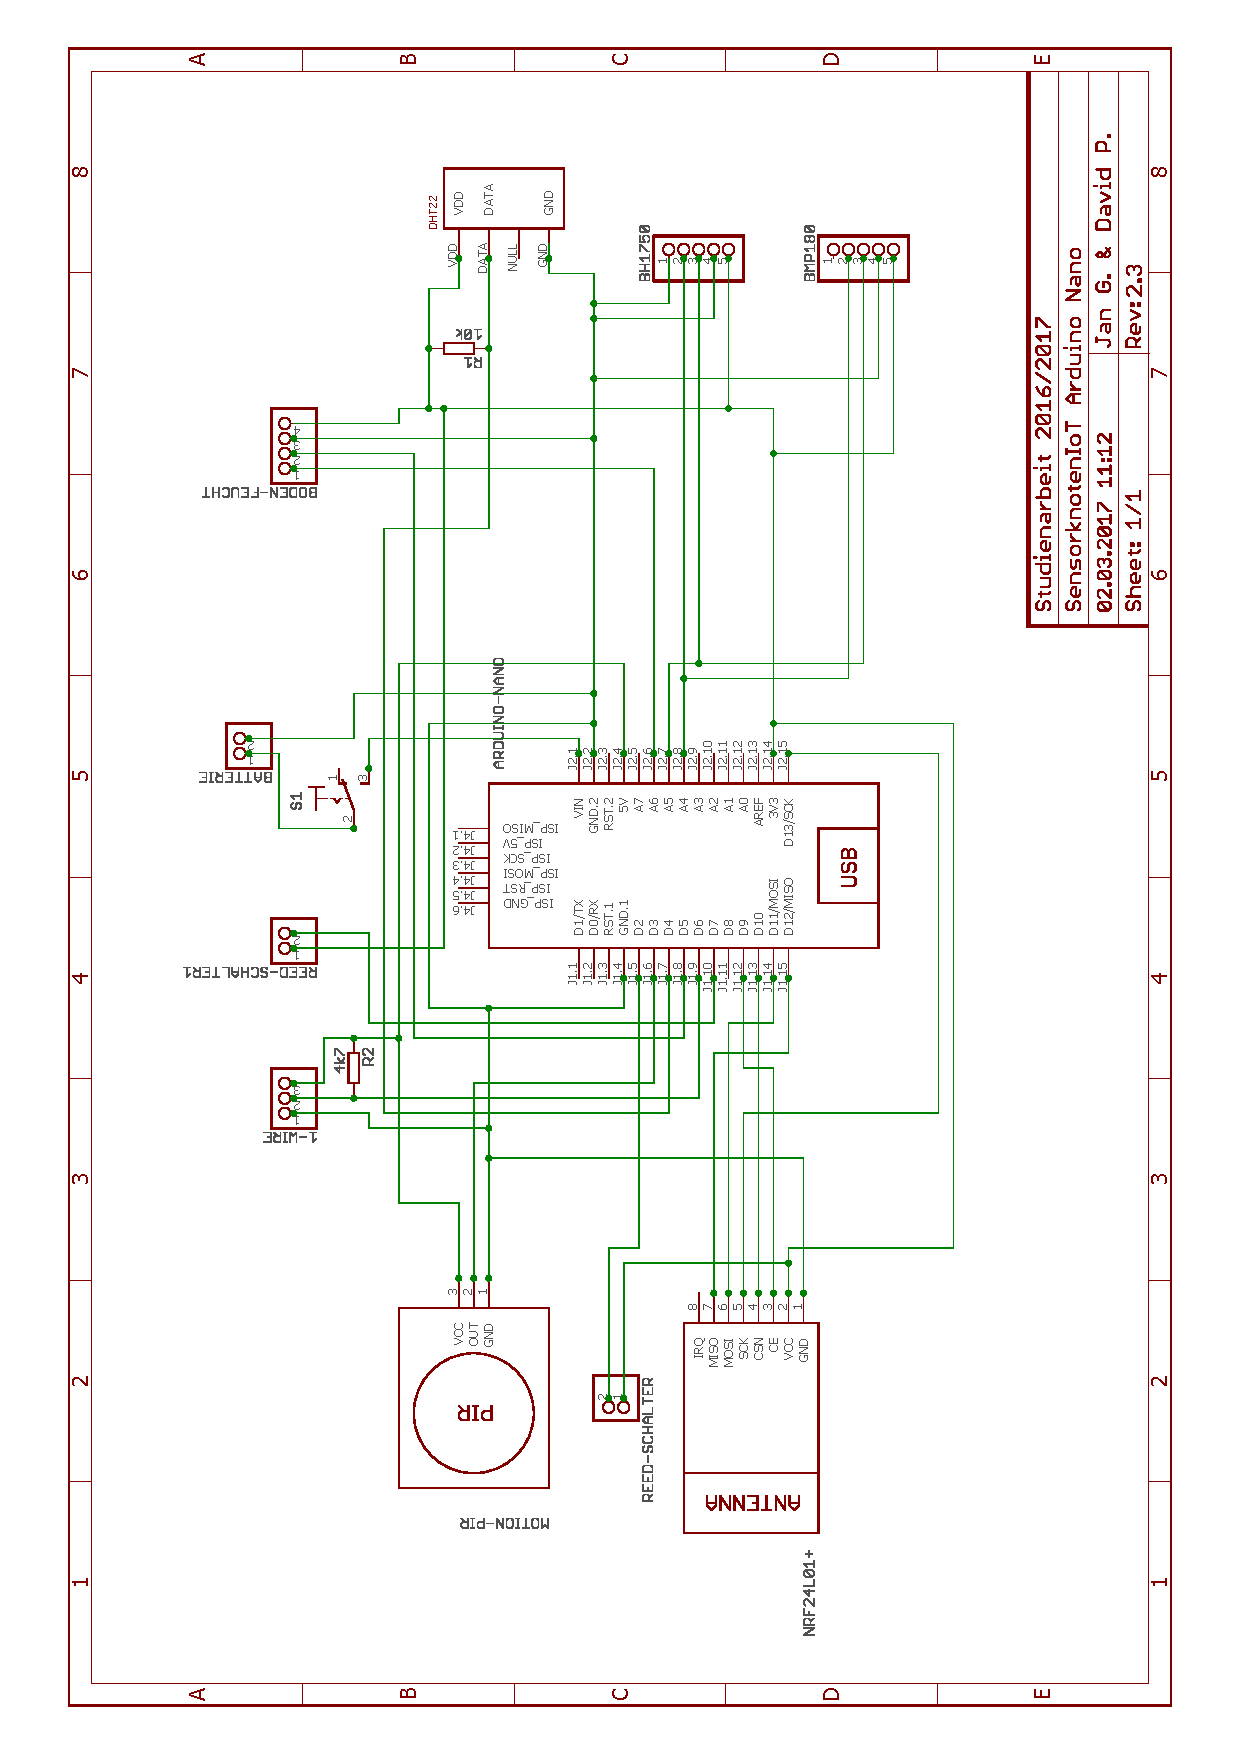
\includepdf[pages=-]{bilder/ArduinoNano-rotated.pdf}
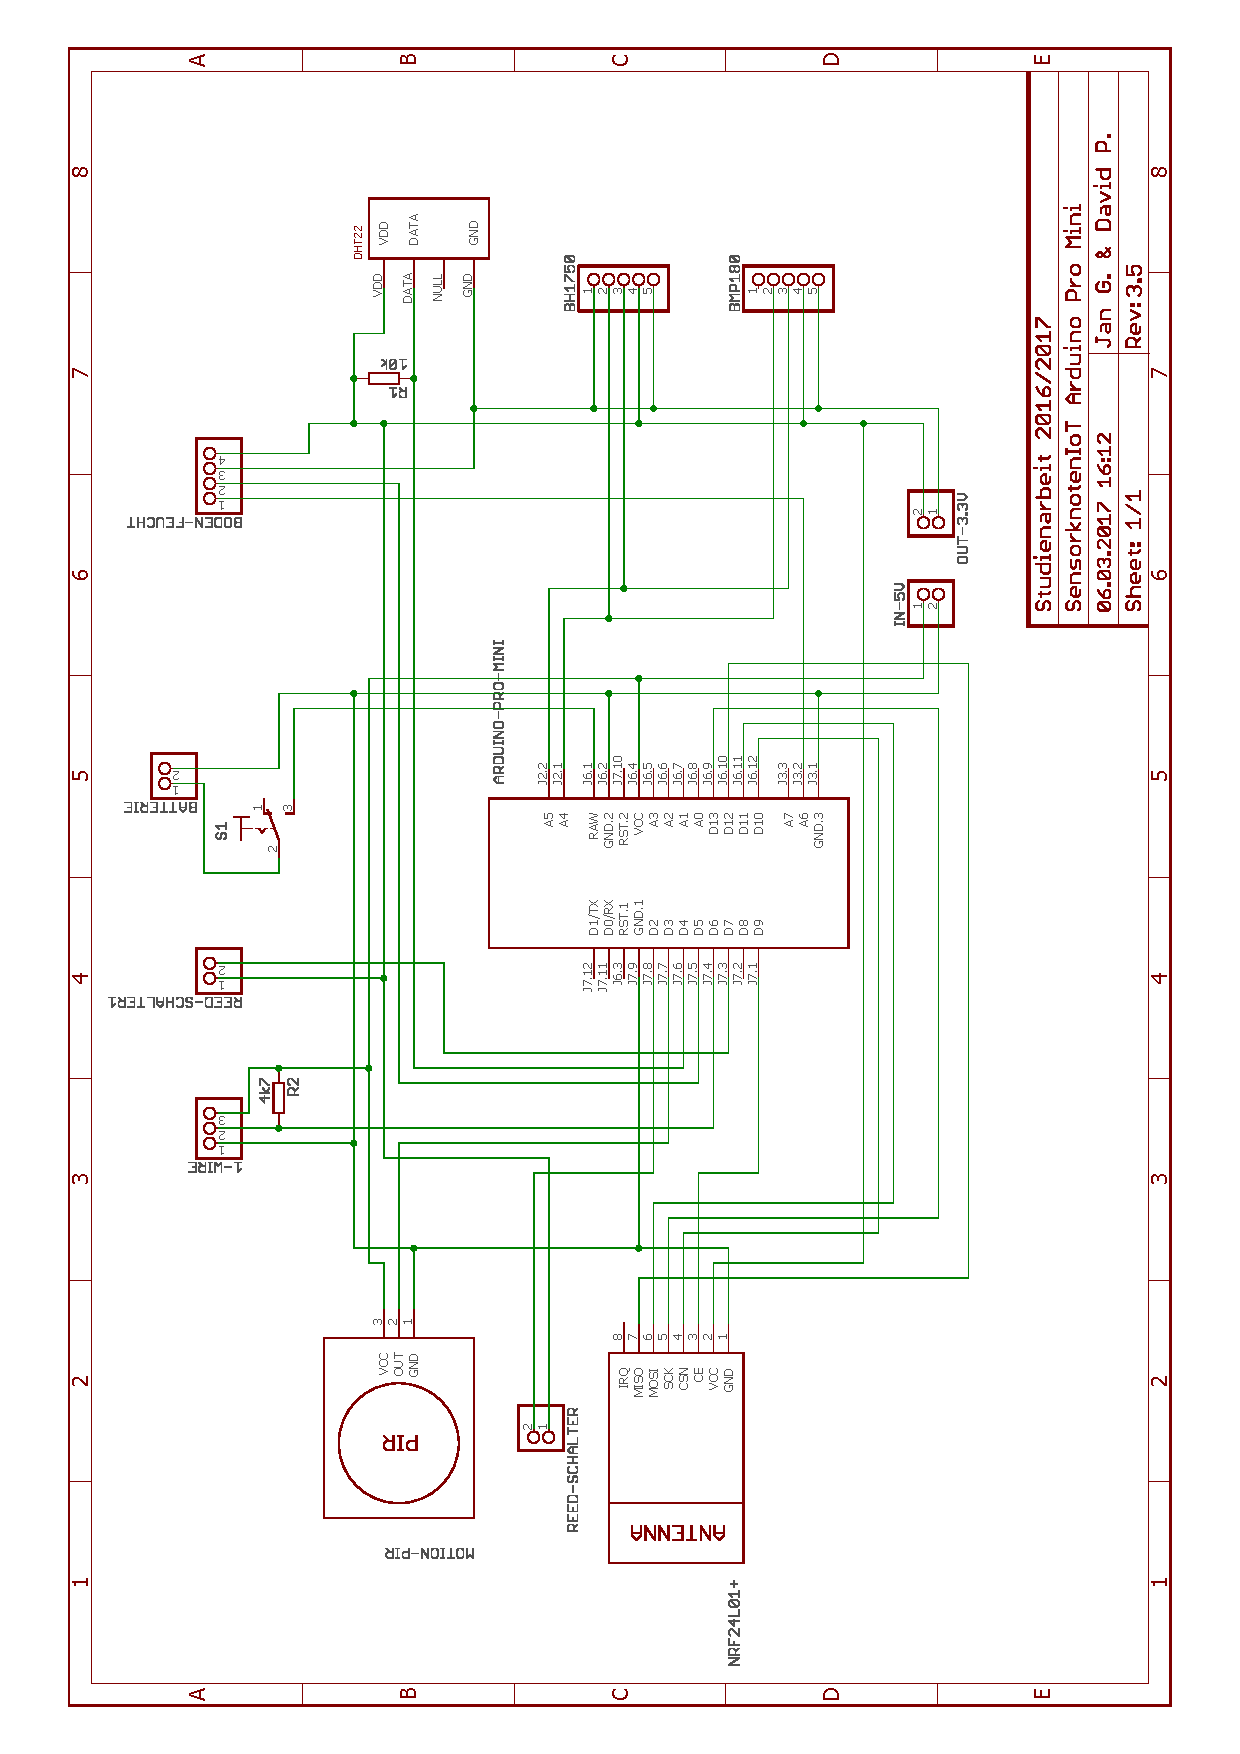
\includepdf[pages=-]{bilder/ArduinoProMini-rotated.pdf}
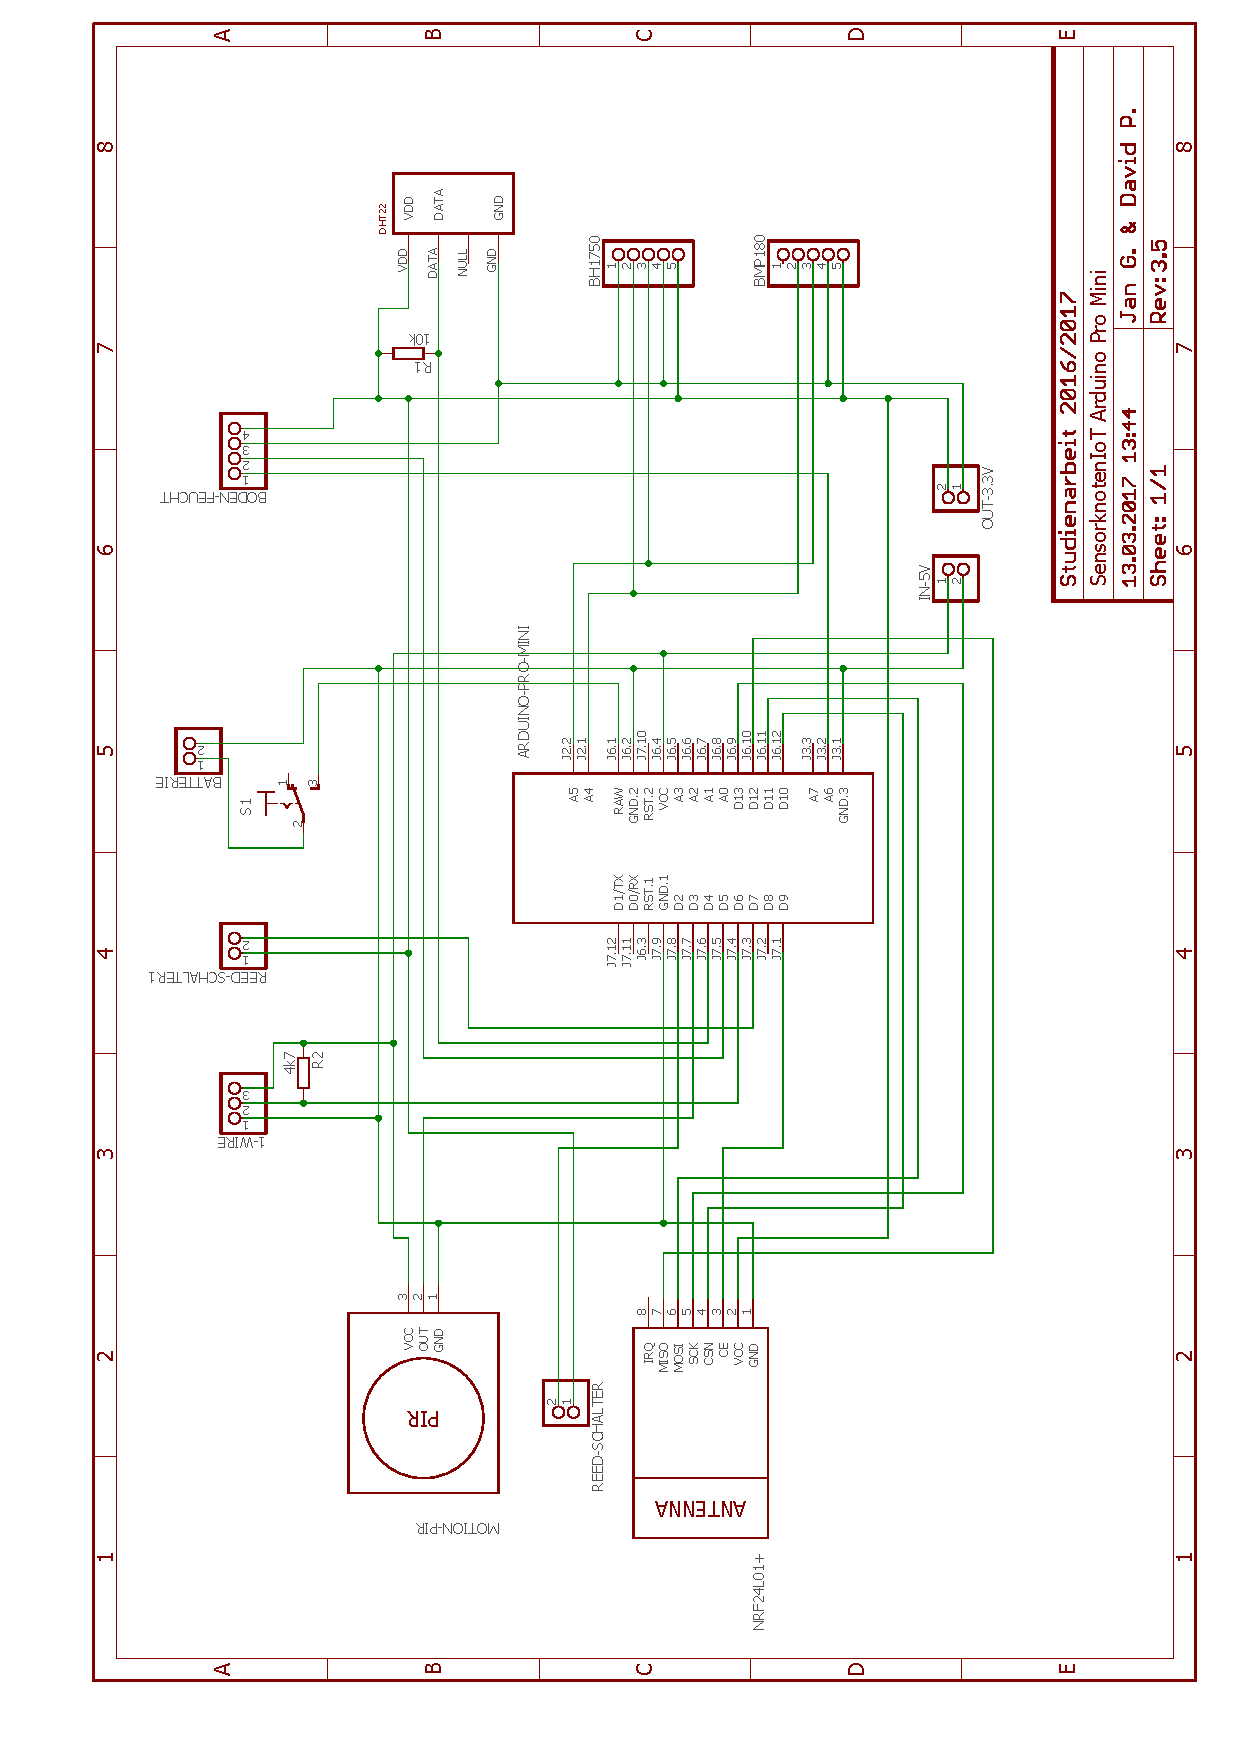
\includepdf[pages=-]{bilder/ArduinoProMiniUeberarbeitet-rotated.pdf}

\newpage
%\addcontentsline{toc}{chapter}{Liste der ToDo's}
%\listoftodos[Liste der ToDo's]



\end{document}

